%%%%%%%%%%%%%%%%%
% Configuration %
%%%%%%%%%%%%%%%%%

\documentclass[10pt, a4paper, twocolumn]{IEEEconf}
\usepackage{amsmath}
\usepackage{amssymb}
\usepackage{mathtools}
\usepackage{csquotes}
\usepackage{xurl}
\urlstyle{rm}
\usepackage[super,comma,sort&compress]{natbib}
%\usepackage[authoryear,comma,sort&compress]{natbib}
\bibliographystyle{unsrtnat}
\usepackage{abstract}
\renewcommand{\abstractnamefont}{\normalfont\bfseries}
\renewcommand{\abstracttextfont}{\normalfont\itshape}
\usepackage{lipsum}
\usepackage{booktabs}
\usepackage{geometry}
\geometry{top=1cm,bottom=1.5cm,left=2cm,right=2cm,includehead,includefoot}
\setlength{\columnsep}{7mm} % Column separation width
\renewcommand*{\thefootnote}{\roman{footnote}}
\renewcommand*{\bibfont}{\raggedright}
\usepackage{float}
\usepackage{graphicx}
\usepackage{subcaption}
\usepackage{bm}
\raggedbottom
\usepackage[bottom]{footmisc}
\interfootnotelinepenalty=100 % Default 100, increase to reduce footnote splitting.
\newcommand\nothing{}
\usepackage{afterpage}

% Inline equations: https://tex.stackexchange.com/a/78582/178803
\makeatletter
\newcommand*{\inlineequation}[2][]{%
  \begingroup
    % Put \refstepcounter at the beginning, because
    % package `hyperref' sets the anchor here.
    \refstepcounter{equation}%
    \ifx\\#1\\%
    \else
      \label{#1}%
    \fi
    % prevent line breaks inside equation
    \relpenalty=10000 %
    \binoppenalty=10000 %
    \ensuremath{%
      % \displaystyle % larger fractions, ...
      #2%
    }%
    ~\@eqnnum
  \endgroup
}

% https://tex.stackexchange.com/a/226719/178803
\newcommand{\oneraggedpage}{\let\mytextbottom\@textbottom
  \let\mytexttop\@texttop
  \raggedbottom
  \afterpage{%
  \global\let\@textbottom\mytextbottom
  \global\let\@texttop\mytexttop}}

% Use these commands to go ragged for one page after the commands:
%\clearpage
%\oneraggedpage

\makeatother

%%%%%%%%%%%%%%
% References %
%%%%%%%%%%%%%%

\begin{filecontents}{value_based_prioritization.bib}

@InCollection{scientific-method,
  author       = {Andersen, Hanne and Hepburn, Brian},
  title        = {Scientific Method},
  booktitle    = {The Stanford Encyclopedia of Philosophy},
  editor       = {Edward N. Zalta},
  year         = {2016},
  edition      = {Summer 2016},
  publisher    = {Metaphysics Research Lab, Stanford University},
  note         = {\url{https://plato.stanford.edu/archives/sum2016/entries/scientific-method/}},
}

@article{martela2016three,
  title        = {The three meanings of meaning in life: Distinguishing coherence, purpose, and significance},
  author       = {Martela, Frank and Steger, Michael F},
  journal      = {The Journal of Positive Psychology},
  volume       = {11},
  number       = {5},
  pages        = {531--545},
  year         = {2016},
  publisher    = {Taylor \& Francis},
  note         = {\url{https://doi.org/10.1080/17439760.2015.1137623}},
}

@book{huemer2007ethical,
  title        = {Ethical Intuitionism},
  author       = {Huemer, Michael},
  year         = {2007},
  publisher    = {Springer},
  note         = {\url{https://spot.colorado.edu/~huemer/5.htm}},
}

@book{huemer2013problem,
  title        = {The Problem of Political Authority},
  author       = {Huemer, Michael},
  year         = {2013},
  publisher    = {Springer},
  note         = {\url{https://spot.colorado.edu/~huemer/1.htm}},
}

@InCollection{value-theory,
  author       = {Schroeder, Mark},
  title        = {Value Theory},
  booktitle    = {The Stanford Encyclopedia of Philosophy},
  editor       = {Edward N. Zalta},
  year         = {2016},
  edition      = {Fall 2016},
  publisher    = {Metaphysics Research Lab, Stanford University},
  note         = {\url{https://plato.stanford.edu/archives/fall2016/entries/value-theory/}},
}

@InCollection{consequentialism,
  author       = {Sinnott-Armstrong, Walter},
  title        = {Consequentialism},
  booktitle    = {The Stanford Encyclopedia of Philosophy},
  editor       = {Edward N. Zalta},
  year         = {2015},
  edition      = {Winter 2015},
  publisher    = {Metaphysics Research Lab, Stanford University},
  note         = {\url{https://plato.stanford.edu/archives/win2015/entries/consequentialism/}},
}

@InCollection{ayn-rand,
  author       = {Badhwar, Neera K. and Long, Roderick T.},
  title        = {Ayn Rand},
  booktitle    = {The Stanford Encyclopedia of Philosophy},
  editor       = {Edward N. Zalta},
  year         = {2017},
  edition      = {Fall 2017},
  publisher    = {Metaphysics Research Lab, Stanford University},
  note         = {\url{https://plato.stanford.edu/archives/fall2017/entries/ayn-rand/}},
}

@InCollection{religion-morality,
  author       = {Hare, John},
  title        = {Religion and Morality},
  booktitle    = {The Stanford Encyclopedia of Philosophy},
  editor       = {Edward N. Zalta},
  year         = {2014},
  edition      = {Winter 2014},
  publisher    = {Metaphysics Research Lab, Stanford University},
  note         = {\url{https://plato.stanford.edu/archives/win2014/entries/religion-morality/}},
}

@InCollection{morality-biology,
  author       = {FitzPatrick, William},
  title        = {Morality and Evolutionary Biology},
  booktitle    = {The Stanford Encyclopedia of Philosophy},
  editor       = {Edward N. Zalta},
  year         = {2016},
  edition      = {Spring 2016},
  publisher    = {Metaphysics Research Lab, Stanford University},
  note         = {\url{https://plato.stanford.edu/archives/spr2016/entries/morality-biology/}},
}

@InCollection{epicurus,
  author       = {Konstan, David},
  title        = {Epicurus},
  booktitle    = {The Stanford Encyclopedia of Philosophy},
  editor       = {Edward N. Zalta},
  year         = {2018},
  edition      = {Summer 2018},
  publisher    = {Metaphysics Research Lab, Stanford University},
  note         = {\url{https://plato.stanford.edu/archives/sum2018/entries/epicurus/}},
}

@InCollection{stoicism,
  author       = {Baltzly, Dirk},
  title        = {Stoicism},
  booktitle    = {The Stanford Encyclopedia of Philosophy},
  editor       = {Edward N. Zalta},
  year         = {2018},
  edition      = {Summer 2018},
  publisher    = {Metaphysics Research Lab, Stanford University},
  note         = {\url{https://plato.stanford.edu/archives/sum2018/entries/stoicism/}},
}

@InCollection{rawls,
  author       = {Wenar, Leif},
  title        = {John Rawls},
  booktitle    = {The Stanford Encyclopedia of Philosophy},
  editor       = {Edward N. Zalta},
  year         = {2017},
  edition      = {Spring 2017},
  publisher    = {Metaphysics Research Lab, Stanford University},
  note         = {\url{https://plato.stanford.edu/archives/spr2017/entries/rawls/}},
}

@InCollection{communitarianism,
  author       = {Bell, Daniel},
  title        = {Communitarianism},
  booktitle    = {The Stanford Encyclopedia of Philosophy},
  editor       = {Edward N. Zalta},
  year         = {2016},
  edition      = {Summer 2016},
  publisher    = {Metaphysics Research Lab, Stanford University},
  note         = {\url{https://plato.stanford.edu/archives/sum2016/entries/communitarianism/}},
}

@article{weinstein2009qalys,
  title        = {{QALYs: the basics}},
  author       = {Weinstein, Milton C and Torrance, George and McGuire, Alistair},
  journal      = {Value in health},
  volume       = {12},
  pages        = {S5--S9},
  year         = {2009},
  publisher    = {Wiley Online Library},
  note         = {\url{https://doi.org/10.1111/j.1524-4733.2009.00515.x}},
}

@article{wit2012all,
  title        = {‘All models are wrong...’: an introduction to model uncertainty},
  author       = {Wit, Ernst and Heuvel, Edwin van den and Romeijn, Jan-Willem},
  journal      = {Statistica Neerlandica},
  volume       = {66},
  number       = {3},
  pages        = {217--236},
  year         = {2012},
  publisher    = {Wiley Online Library},
  note         = {\url{https://doi.org/10.1111/j.1467-9574.2012.00530.x}},
}

@misc{centers2017underlying,
  title        = {{Underlying Cause of Death 1999-2017}},
  author       = {{Centers for Disease Control and Prevention and National Center for Health Statistics}},
  howpublished = {\url{https://wonder.cdc.gov/ucd-icd10.html}},
  note         = {Accessed: 2019-03-01},
}

@book{icd10vol1,
  title        = {International statistical classification of diseases and related health problems},
  author       = {World Health Organization},
  year         = {2016},
  publisher    = {World Health Organization},
  edition      = {10th},
  volume       = {1},
  note         = {\url{https://apps.who.int/iris/bitstream/handle/10665/246208/9789241549165-V1-eng.pdf}},
}

@book{icd10vol2,
  title        = {International statistical classification of diseases and related health problems},
  author       = {World Health Organization},
  year         = {2010},
  publisher    = {World Health Organization},
  edition      = {10th},
  volume       = {2},
  note         = {\url{https://www.who.int/classifications/icd/ICD10Volume2_en_2010.pdf}},
}

@book{icd10vol3,
  title        = {International statistical classification of diseases and related health problems},
  author       = {World Health Organization},
  year         = {2016},
  publisher    = {World Health Organization},
  edition      = {10th},
  volume       = {3},
  note         = {\url{https://apps.who.int/iris/bitstream/handle/10665/246208/9789241549165-V3-eng.pdf}},
}

@article{anderson2004model,
  title        = {Model selection and multi-model inference},
  author       = {Anderson, DR and Burnham, K},
  journal      = {Second. NY: Springer-Verlag},
  year         = {2004},
  note         = {\url{https://cds.cern.ch/record/1608735/files/9780387953649_TOC.pdf}},
}

@article{burnham2004multimodel,
  title        = {Multimodel inference: understanding AIC and BIC in model selection},
  author       = {Burnham, Kenneth P and Anderson, David R},
  journal      = {Sociological methods \& research},
  volume       = {33},
  number       = {2},
  pages        = {261--304},
  year         = {2004},
  publisher    = {Sage Publications Sage CA: Thousand Oaks, CA},
  note         = {\url{https://doi.org/10.1177/0049124104268644}},
}

@book{berk2004regression,
  title        = {Regression analysis: A constructive critique},
  author       = {Berk, Richard A},
  volume       = {11},
  year         = {2004},
  publisher    = {Sage},
}

@book{hyndman2018forecasting,
  title        = {Forecasting: principles and practice},
  author       = {Hyndman, Rob J and Athanasopoulos, George},
  year         = {2018},
  publisher    = {OTexts},
  note         = {\url{https://otexts.com/fpp2/}},
}

@article{clemen1989combining,
  title        = {Combining forecasts: A review and annotated bibliography},
  author       = {Clemen, Robert T},
  journal      = {International journal of forecasting},
  volume       = {5},
  number       = {4},
  pages        = {559--583},
  year         = {1989},
  publisher    = {Elsevier},
  note         = {\url{https://doi.org/10.1016/0169-2070(89)90012-5}},
}

@article{taylor2018forecasting,
  title        = {Forecasting at scale},
  author       = {Taylor, Sean J and Letham, Benjamin},
  journal      = {The American Statistician},
  volume       = {72},
  number       = {1},
  pages        = {37--45},
  year         = {2018},
  publisher    = {Taylor \& Francis},
  note         = {\url{https://doi.org/10.1080/00031305.2017.1380080}},
}

@article{makridakis2018m4,
  title        = {The M4 Competition: Results, findings, conclusion and way forward},
  author       = {Makridakis, Spyros and Spiliotis, Evangelos and Assimakopoulos, Vassilios},
  journal      = {International Journal of Forecasting},
  volume       = {34},
  number       = {4},
  pages        = {802--808},
  year         = {2018},
  publisher    = {Elsevier},
  note         = {\url{https://doi.org/10.1016/j.ijforecast.2018.06.001}},
}

@misc{censusestimates19001999,
  title        = {{Historical National Population Estimates}},
  author       = {{U.S. Census Bureau}},
  howpublished = {\url{https://www2.census.gov/programs-surveys/popest/tables/1900-1980/national/totals/popclockest.txt}},
  note         = {Accessed: 2019-03-01},
}

@misc{worldbankopendata,
  title        = {{World Bank Open Data: United States SP.POP.TOTL}},
  author       = {{World Bank}},
  howpublished = {\url{http://api.worldbank.org/v2/en/country/USA?downloadformat=csv}},
  note         = {Accessed: 2019-03-01},
}

@misc{nbermortality,
  title        = {{Mortality Data: Vital Statistics NCHS' Multiple Cause of Death Data, 1959-2017}},
  author       = {{The National Bureau of Economic Research}},
  howpublished = {\url{https://www.nber.org/data/vital-statistics-mortality-data-multiple-cause-of-death.html}},
  note         = {Accessed: 2019-03-01},
}

@misc{icdcomparabilityratios,
  title        = {{A Guide to State Implementation of ICD-10 for Mortality; Part II: Applying Comparability Ratios}},
  author       = {{Centers for Disease Control and Prevention and National Center for Health Statistics\nothing}},
  howpublished = {\url{https://www.cdc.gov/nchs/data/statab/document-for-the-states.pdf}},
  note         = {Accessed: 2019-03-01},
}

@article{mathers2006projections,
  title        = {Projections of global mortality and burden of disease from 2002 to 2030},
  author       = {Mathers, Colin D and Loncar, Dejan},
  journal      = {PLoS medicine},
  volume       = {3},
  number       = {11},
  pages        = {e442},
  year         = {2006},
  publisher    = {Public Library of Science},
  note         = {\url{https://doi.org/10.1371/journal.pmed.0030442}},
}

@misc{uspopulation19002001,
  title        = {{United States Population by Age, Race, and Sex, 1900-90, and 1991-2001}},
  author       = {{Centers for Disease Control and Prevention and National Center for Health Statistics\nothing\nothing}},
  howpublished = {\url{https://www.cdc.gov/nchs/nvss/mortality/historical_population.htm}},
  note         = {Accessed: 2019-03-01},
}

@misc{uslcod19001998,
  title        = {{Leading Causes of Death, 1900-1998}},
  author       = {{Centers for Disease Control and Prevention and National Center for Health Statistics\nothing\nothing\nothing}},
  howpublished = {\url{https://www.cdc.gov/nchs/nvss/mortality_historical_data.htm}},
  note         = {Accessed: 2019-03-01},
}

@book{lopez2006global,
  title        = {Global burden of disease and risk factors},
  author       = {Lopez, Alan D and Mathers, Colin D and Ezzati, Majid and Jamison, Dean T and Murray, Christopher JL},
  year         = {2006},
  publisher    = {The World Bank},
  note         = {\url{https://openknowledge.worldbank.org/bitstream/handle/10986/7039/364010PAPER0Gl101OFFICIAL0USE0ONLY1.pdf}},
}

@article{world2009guide,
  title        = {{WHO guide to identifying the economic consequences of disease and injury}},
  author       = {World Health Organization and others},
  year         = {2009},
  publisher    = {World Health Organization},
  note         = {\url{https://www.who.int/choice/publications/d_economic_impact_guide.pdf}},
}

@misc{givewellcosteffectiveness,
  title        = {{Some considerations against more investment in cost-effectiveness estimates}},
  author       = {{GiveWell.org}},
  howpublished = {\url{https://blog.givewell.org/2011/11/04/some-considerations-against-more-investment-in-cost-effectiveness-estimates/}},
  note         = {Accessed: 2019-03-01},
}

@book{jamison2017disease,
  title        = {Disease Control Priorities, (Volume 9): Improving Health and Reducing Poverty},
  author       = {Jamison, Dean T and Gelband, Hellen and Horton, Susan and Jha, Prabhat and Laxminarayan, Ramanan and Mock, Charles N and Nugent, Rachel},
  year         = {2017},
  publisher    = {The World Bank},
  note         = {\url{https://openknowledge.worldbank.org/bitstream/handle/10986/28877/9781464805271.pdf}},
}

@article{neumann2018comparing,
  title        = {Comparing the cost-per-QALYs gained and cost-per-DALYs averted literatures},
  author       = {Neumann, Peter J and Anderson, Jordan E and Panzer, Ari D and Pope, Elle F and D'Cruz, Brittany N and Kim, David D and Cohen, Joshua T},
  journal      = {Gates open research},
  volume       = {2},
  year         = {2018},
  publisher    = {Gates Foundation-Open Access},
  note         = {\url{https://doi.org/10.12688/gatesopenres.12786.2}},
}

@article{bostrom2013existential,
  title        = {Existential risk prevention as global priority},
  author       = {Bostrom, Nick},
  journal      = {Global Policy},
  volume       = {4},
  number       = {1},
  pages        = {15--31},
  year         = {2013},
  publisher    = {Wiley Online Library},
  note         = {\url{https://www.existential-risk.org/concept.pdf}},
}

@book{macaskill2015doing,
  title        = {Doing good better: Effective altruism and a radical new way to make a difference},
  author       = {MacAskill, William},
  year         = {2015},
  publisher    = {Guardian Faber Publishing},
}

@misc{whomortality,
  title        = {{WHO Mortality Database}},
  author       = {{World Health Organization}},
  howpublished = {\url{https://www.who.int/healthinfo/statistics/mortality_rawdata/en/}},
  note         = {Accessed: 2019-03-01},
}

@article{de200625,
  title        = {25 years of time series forecasting},
  author       = {De Gooijer, Jan G and Hyndman, Rob J},
  journal      = {International journal of forecasting},
  volume       = {22},
  number       = {3},
  pages        = {443--473},
  year         = {2006},
  publisher    = {Elsevier},
  note         = {\url{https://doi.org/10.1016/j.ijforecast.2006.01.001}},
}

@misc{tashman1991automatic,
  title        = {{Automatic forecasting software: A survey and evaluation}},
  author       = {Tashman, Leonard J and Leach, Michael L},
  year         = {1991},
  publisher    = {Elsevier},
  note         = {\url{https://doi.org/10.1016/0169-2070(91)90055-Z}},
}

@book{hyndman2008forecasting,
  title        = {Forecasting with exponential smoothing: the state space approach},
  author       = {Hyndman, Rob and Koehler, Anne B and Ord, J Keith and Snyder, Ralph D},
  year         = {2008},
  publisher    = {Springer Science \& Business Media},
  note         = {\url{http://www.exponentialsmoothing.net/}},
}

@InCollection{sep-rationalism-empiricism,
  author       = {Markie, Peter},
  title        = {Rationalism vs. Empiricism},
  booktitle    = {The Stanford Encyclopedia of Philosophy},
  editor       = {Edward N. Zalta},
  year         = {2017},
  edition      = {Fall 2017},
  publisher    = {Metaphysics Research Lab, Stanford University},
  note         = {\url{https://plato.stanford.edu/archives/fall2017/entries/rationalism-empiricism/}},
}

@article{huemer2012praise,
  title        = {In praise of passivity},
  author       = {Huemer, Michael},
  journal      = {Studia Humana},
  volume       = {1},
  number       = {2},
  pages        = {12--28},
  year         = {2012},
  note         = {\url{http://studiahumana.com/pliki/wydania/In\%20Praise\%20of\%20Passivity.pdf}},
}

@article{anderson2001comparability,
  title        = {Comparability of Cause of Death between ICD-9 and ICD-10: Preliminary Estimates},
  author       = {Anderson, Robert N and Mini{\~n}o, Arialdi M and Hoyert, Donna L and Rosenberg, Harry M},
  year         = {2001},
  note         = {\url{https://www.cdc.gov/nchs/data/nvsr/nvsr49/nvsr49_02.pdf}},
}

@book{baumeister1991meanings,
  title        = {Meanings of life},
  author       = {Baumeister, Roy F},
  year         = {1991},
  publisher    = {Guilford Press},
}

@book{oades2017wiley,
  title        = {The Wiley Blackwell handbook of the psychology of positivity and strengths-based approaches at work},
  author       = {Oades, Lindsay G and Steger, Michael and Delle Fave, Antonelle and Passmore, Jonathan},
  year         = {2017},
  publisher    = {John Wiley \& Sons},
}

@incollection{steger2013experiencing,
  title        = {Experiencing meaning in life: Optimal functioning at the nexus of well-being, psychopathology, and spirituality},
  author       = {Steger, Michael F},
  booktitle    = {The human quest for meaning},
  pages        = {211--230},
  year         = {2013},
  publisher    = {Routledge},
}

@article{dik2009calling,
  title        = {Calling and vocation in career counseling: Recommendations for promoting meaningful work.},
  author       = {Dik, Bryan J and Duffy, Ryan D and Eldridge, Brandy M},
  journal      = {Professional Psychology: Research and Practice},
  volume       = {40},
  number       = {6},
  pages        = {625},
  year         = {2009},
  publisher    = {American Psychological Association},
  note         = {\url{https://doi.org/10.1037/a0015547}},
}

@article{zikic2009job,
  title        = {Job search and social cognitive theory: The role of career-relevant activities},
  author       = {Zikic, Jelena and Saks, Alan M},
  journal      = {Journal of Vocational Behavior},
  volume       = {74},
  number       = {1},
  pages        = {117--127},
  year         = {2009},
  publisher    = {Elsevier},
  note         = {\url{https://doi.org/10.1016/j.jvb.2008.11.001}},
}

@article{steger2006meaning,
  title        = {The meaning in life questionnaire: Assessing the presence of and search for meaning in life.},
  author       = {Steger, Michael F and Frazier, Patricia and Oishi, Shigehiro and Kaler, Matthew},
  journal      = {Journal of counseling psychology},
  volume       = {53},
  number       = {1},
  pages        = {80},
  year         = {2006},
  publisher    = {American Psychological Association},
  note         = {\url{https://doi.org/10.1037/0022-0167.53.1.80}},
}

@book{seligman2006learned,
  title        = {Learned optimism: How to change your mind and your life},
  author       = {Seligman, Martin EP},
  year         = {2006},
  publisher    = {Vintage},
}

@book{frankl1985man,
  title        = {Man's search for meaning},
  author       = {Frankl, Viktor E},
  year         = {1985},
  publisher    = {Simon and Schuster},
}

@article{baumeister2013some,
  title        = {Some key differences between a happy life and a meaningful life},
  author       = {Baumeister, Roy F and Vohs, Kathleen D and Aaker, Jennifer L and Garbinsky, Emily N},
  journal      = {The journal of positive psychology},
  volume       = {8},
  number       = {6},
  pages        = {505--516},
  year         = {2013},
  publisher    = {Taylor \& Francis},
  note         = {\url{https://doi.org/10.1080/17439760.2013.830764}},
}

@article{park2013assessing,
  title        = {Assessing meaning and meaning making in the context of stressful life events: Measurement tools and approaches},
  author       = {Park, Crystal L and George, Login S},
  journal      = {The Journal of Positive Psychology},
  volume       = {8},
  number       = {6},
  pages        = {483--504},
  year         = {2013},
  publisher    = {Taylor \& Francis},
}

@article{george2013meaning,
  title        = {Are meaning and purpose distinct? An examination of correlates and predictors},
  author       = {George, Login S and Park, Crystal L},
  journal      = {The Journal of Positive Psychology},
  volume       = {8},
  number       = {5},
  pages        = {365--375},
  year         = {2013},
  publisher    = {Taylor \& Francis},
  note         = {\url{https://doi.org/10.1080/17439760.2013.805801}},
}

@article{allan2015meaning,
  title        = {Meaning in life and work: A developmental perspective},
  author       = {Allan, Blake A and Duffy, Ryan D and Douglass, Richard},
  journal      = {The Journal of Positive Psychology},
  volume       = {10},
  number       = {4},
  pages        = {323--331},
  year         = {2015},
  publisher    = {Taylor \& Francis},
  note         = {\url{https://doi.org/10.1080/17439760.2014.950180}},
}

@book{dik2012make,
  title        = {Make your job a calling: How the psychology of vocation can change your life at work},
  author       = {Dik, Bryan J and Duffy, Ryan D},
  year         = {2012},
  publisher    = {Templeton Foundation Press},
}

@article{steger2009if,
  title        = {If one is looking for meaning in life, does it help to find meaning in work?},
  author       = {Steger, Michael F and Dik, Bryan J},
  journal      = {Applied Psychology: Health and Well-Being},
  volume       = {1},
  number       = {3},
  pages        = {303--320},
  year         = {2009},
  publisher    = {Wiley Online Library},
  note         = {\url{https://doi.org/10.1111/j.1758-0854.2009.01018.x}},
}

@article{wong2010meaning,
  title        = {Meaning therapy: An integrative and positive existential psychotherapy},
  author       = {Wong, Paul TP},
  journal      = {Journal of Contemporary Psychotherapy},
  volume       = {40},
  number       = {2},
  pages        = {85--93},
  year         = {2010},
  publisher    = {Springer},
  note         = {\url{https://doi.org/10.1007/s10879-009-9132-6}},
}

@article{heintzelman2013knowing,
  title        = {On knowing more than we can tell: Intuitive processes and the experience of meaning},
  author       = {Heintzelman, Samantha J and King, Laura A},
  journal      = {The Journal of Positive Psychology},
  volume       = {8},
  number       = {6},
  pages        = {471--482},
  year         = {2013},
  publisher    = {Taylor \& Francis},
  note         = {\url{https://doi.org/10.1080/17439760.2013.830758}},
}

\end{filecontents}

\usepackage{hyperref}
\hypersetup{colorlinks=true, urlcolor=blue, linkcolor=blue, citecolor=blue}

\begin{document}
\flushbottom
\title{Value-Based Prioritization: A method for choosing meaningful work\thanks{\url{https://github.com/freeradical13/ValueBasedPrioritization}}}

\author{Kevin Grigorenko\thanks{\href{mailto:kevin@myplaceonline.com}{kevin@myplaceonline.com}}}

\newcommand{\abstractText}{\noindent
A method is proposed to use value theory to select and quantitatively prioritize actions to accomplish a goal.
Actions are relatively ranked based on some quantitative measurement(s) as called for by the value theory.
This ranking is transformed by a set of functions which scale up and down each action's relative score based on other relevant measurements and subjective opinions.
The resulting list provides a prioritized relative ranking of actions that should be pursued in a particular order.
This method is applied to the example of choosing meaningful work using an example value system based on the goal to reduce human suffering.
}

%%%%%%%%%%%%
% Abstract %
%%%%%%%%%%%%

\twocolumn[
  \begin{@twocolumnfalse}
    \maketitle
    \begin{center}
      \date{\today}
    \end{center}
    \begin{abstract}
      \abstractText
      \newline
      \newline
    \end{abstract}
    \tableofcontents
  \end{@twocolumnfalse}
]

\saythanks

% Page numbers:
\thispagestyle{plain}
\pagestyle{plain}

%%%%%%%%%%%
% Article %
%%%%%%%%%%%

\clearpage

\section{Background}

Why should a particular goal be pursued (\enquote{Why})?
Given a goal, what actions should be pursued to best accomplish that goal (\enquote{What})?
Given an action, how should that action be pursued (\enquote{How})?

\subsection{Existing research}

To exemplify these questions, the issue of choosing meaningful work is selected. One field that investigates the question of meaningful work is psychology, largely in specialties such as positive and vocational psychology.

Although there are significant efforts to establish the importance of a meaningful life \citep{martela2016three,baumeister1991meanings,frankl1985man,baumeister2013some,park2013assessing,allan2015meaning,heintzelman2013knowing} and meaningful work \citep{steger2013experiencing,dik2009calling,oades2017wiley,steger2009if}, calling \citep{dik2012make}, or purpose \citep{george2013meaning}, and survey perceptions of meaningful work \citep{steger2006meaning}, efforts to provide detailed methods of choosing such meaningful work are largely confined to vague techniques such as evaluations of psychological profiles for signature strengths \citep{seligman2006learned}, career counseling \citep{dik2009calling} or therapy \citep{wong2010meaning}, and job search training \citep{zikic2009job}. These approaches are important prerequisites but their less quantitative and less explicit nature make them difficult to evaluate, generalize, and improve.

\section{Value-Based Prioritization}

This article proposes that value theory usually best scopes \enquote{Why} and \enquote{What} and the scientific method usually best answers \enquote{How}.
A method called Value-Based Prioritization is developed to answer the \enquote{What} question:

\begin{equation*}
  \begin{gathered}
    \textrm{Why: } \textit{Value Theory} \\
    \downarrow \\
    \textrm{What: } \textit{\textit{Value-Based Prioritization}} \\
    \downarrow \\
    \textrm{How: } \textit{Scientific Method}
  \end{gathered}
\end{equation*}

\subsection{Why a Goal?}

\enquote{Why a Goal?} is usually best scoped using value systems because they are evaluative by nature \citep{value-theory}.
Comparing value systems is left as an (lifelong) exercise for the reader\footnote{Example value systems include intuitionism \citep{huemer2007ethical}, consequentialism \citep{consequentialism}, evolutionary biology \citep{morality-biology}, religion \citep{religion-morality}, epicureanism \citep{epicurus}, stoicism \citep{stoicism}, political liberalism \citep{rawls}, anarcho-capitalism \citep{huemer2013problem}, communitarianism \citep{communitarianism}, objectivism \citep{ayn-rand}, etc.}.

\subsection{What Actions?}

\enquote{What Actions?} is usually best scoped by prioritizing actions because actions usually have differing effect sizes and time is limited.
It follows from the value system used to answer \enquote{Why} that the same value system is used primarily to evaluate the priority of each action.

Value-Based Prioritization builds a quantitative prioritization model based on predicted effect sizes.
Raw prioritization scores are further scaled by contextual factors such as implementation time, cost, risk, and other judgments.

\subsection{How to do an Action?}

Given answers to \enquote{Why?} and \enquote{What?}, how to implement actions is usually best answered with the scientific method \citep{scientific-method,sep-rationalism-empiricism}: observations are made and rational thought is used to generate hypotheses, hypotheses are tested with experiments, and successful experiments lead to theories and results.

\subsection{Method}

A \textit{value system} \inlineequation[value-system]{V} generates a \textit{goal} \inlineequation[goal]{G(t)} (for some time $t$) and a set of \textit{mutually exclusive potential actions} $A(t)$:

\begin{equation}\label{potential-actions}
  \begin{gathered}
    A(t) = \{A_1(t), \ldots, A_N(t)\}, \\
    N > 1
  \end{gathered}
\end{equation}

An action's \textit{estimated relative accomplishment amount} $B(A(t))$ is an action's expected \textit{relative} (i.e. with respect to other actions) contribution towards accomplishing $G$(t):

\begin{equation}\label{action-amount}
  \begin{gathered}
    B(A(t)) = \mathbb{R}, \\
    0 \leq \mathbb{R} \leq 1
  \end{gathered}
\end{equation}

Thus, $G(t)$ is fully accomplished if all actions are accomplished:

\begin{equation}\label{goal-accomplished}
  G(t) = \sum_{i=1}^{N} B(A_i(t)) = 1
\end{equation}

A \textit{value-based prioritization score} $C(A(t))$ is the result of the product of a set of \textit{value-based prioritization scale functions} \inlineequation[scale-functions]{S = \{S_1, \ldots, S_N\}} multiplied by \eqref{action-amount}:

\begin{equation}\label{prioritization-score}
  \begin{gathered}
    C(A(t)) = B(A(t)) \cdot \prod_{j=1}^{N} S_j(A(t)), \\
    0 \leq S_j(A(t)) \leq 1
  \end{gathered}
\end{equation}

Example scale functions include implementation time, cost, risk, and other judgments.
Ideally, scale functions should be defined before running the model to reduce bias.
The set $S$ always includes the element $S_1(A(t)) = 1$.

A \textit{value-based prioritization} (VBP) $Z(t)$ is a sequence of actions ordered by prioritization score \eqref{prioritization-score} in descending order:

\begin{equation}\label{vbp}
  \begin{gathered}
    Z(t) = (A_1(t), \ldots, A_N(t)), \\
    C(A_1(t)) \geq \ldots \geq C(A_N(t))
  \end{gathered}
\end{equation}

The first $k$ actions in $Z(t)$ should be executed in descending priority/proportion where \inlineequation[how-many-actions]{k} is chosen based on factors such as available concurrency, time, resources, etc.

\subsection{Modeled Value-Based Prioritization}

Historical data may be used to predict actions' estimated relative accomplishment amounts \eqref{action-amount} at a future time \inlineequation[modeled-future-time]{t_F}.

If each action has historical data $D(A)$:

\begin{equation}\label{action-predictors}
  \begin{multlined}
    D(A) = \\
    \shoveleft[0.5cm]{((t_1, D(A,t_1)), \ldots, (t_N, D(A,t_N)))}
  \end{multlined}
\end{equation}

Then, a set of \textit{comparable prediction models} (or forecasting models) \citep{de200625,tashman1991automatic,hyndman2018forecasting,taylor2018forecasting,wit2012all} $R(D(A))$ is applied to each $D(A)$ (e.g. exponential smoothing \citep{hyndman2018forecasting,hyndman2008forecasting}\textsuperscript{,}\footnote{\scriptsize{\url{https://otexts.com/fpp2/expsmooth.html}}}, a generalized additive model [GAM] \citep{taylor2018forecasting}, ARIMA \citep{hyndman2018forecasting}\textsuperscript{,}\footnote{\scriptsize{\url{https://otexts.com/fpp2/arima.html}}}, linear regression \citep{hyndman2018forecasting}\textsuperscript{,}\footnote{\scriptsize{\url{https://otexts.com/fpp2/regression.html}}}, machine learning \citep{makridakis2018m4}, seasonal algorithms such as TBATS \citep{hyndman2018forecasting}\textsuperscript{,}\footnote{\scriptsize{\url{https://otexts.com/fpp2/advanced.html}}}, poisson log-bilinear regression \citep{mathers2006projections}, etc.):

\begin{equation}\label{prediction-models}
  \begin{multlined}
    R(D(A)) =\\
    \{R_1(D(A)), \ldots, R_N(D(A))\}
  \end{multlined}
\end{equation}

The models are compared using a \textit{model selection} algorithm\footnote{\scriptsize{\url{https://otexts.com/fpp2/selecting-predictors.html}}} \inlineequation[model-selection]{L(R(D(A)))} (e.g. smallest Akaike's Information Criterion [AIC], smallest Corrected AIC [AICc], smallest Bayesian Information Criterion [BIC], smallest cross-validation, largest adjusted coefficient of determination [$\bar{R^2}$], etc.).

For each action, $L(R(D(A)))$ produces the \textit{best fitting model} $M(A(t))$ (or a model that's an average of multiple models \citep{clemen1989combining}\textsuperscript{,}\footnote{\scriptsize{\url{https://otexts.com/fpp2/combinations.html}}}).

Each action's $M(A(t_F))$ is used to predict $B(A(t_F))$.

Finally, \textit{modeled value-based prioritization} (MVBP) $Z(t_F)$ is simply \eqref{vbp} with $t_F$:

\begin{equation}\label{modeled-vbp}
  \begin{gathered}
    Z(t_F) = (A_1(t_F), \ldots, A_N(t_F)), \\
    C(A_1(t_F)) \geq \ldots \geq C(A_N(t_F))
  \end{gathered}
\end{equation}

\section{Choosing meaningful work}\label{section-example}

\subsection{Method}

The following example applies modeled value-based prioritization \eqref{modeled-vbp} to the goal of choosing meaningful work.
Every aspect is an example and should be reconsidered.

First, outline the parameters:

\begin{itemize}
  \item \eqref{value-system} $V = $ a value system which answers \enquote{Why work?} with \enquote{To reduce human suffering} which is defined as maximal human suffering: death (more precisely, something like the lack of a potential of life).
  Alternatives include morbidity and disease burden (e.g. Quality-Adjusted Life Years [QALYs] \citep{weinstein2009qalys,lopez2006global}), non-human suffering, cost effectiveness \citep{jamison2017disease,neumann2018comparing,givewellcosteffectiveness}, economic impact \citep{world2009guide}, existential risks \citep{bostrom2013existential}, pre-birth suffering, working to give \citep{macaskill2015doing}, etc.
  \item \eqref{goal} $G(t) = $ eliminate human death.
  \item \eqref{potential-actions} $A(t) = $ the set of actions which would eliminate human death.
  \item \eqref{how-many-actions} $k = $ 1 for a single person (or 2 to hedge the failure of the first action or to add a volunteer activity).
  \item \eqref{modeled-future-time} $t_F = $ 10 years; an average amount of time under normal conditions to integrate into a new career to work on some subset of $A(t)$ (including learning, certification, building experience, networking, etc.).
  \item \eqref{action-predictors} $D(A) = $ time-series data on human death by underlying cause\footnote{\scriptsize{\url{https://www.who.int/topics/mortality/en/}}}.
  \item \eqref{prediction-models} $R(D(A)) = $ exponential smoothing functions using Holt's linear trend method as aggregate models\footnote{\scriptsize{\url{https://otexts.com/fpp2/holt.html}}}\textsuperscript{,}\footnote{\scriptsize{\url{https://otexts.com/fpp2/ets.html}}}\textsuperscript{,}\footnote{\scriptsize{\url{https://www.statsmodels.org/dev/examples/notebooks/generated/exponential_smoothing.html}}} ($ETS(A,M,N)$ and $ETS(A,M_d,N)$ were tested but had bad failure modes, particularly with outliers.):
    \begin{equation*}
      \begin{gathered}
        \{ETS(A,A,N),ETS(A,A_d,N)\},\\
        \phi=0.98
      \end{gathered}
    \end{equation*}
    Commonly used alternative models in all-cause mortality forecasting include poisson log-bilinear regressions\footnote{See Appendix note \ref{mathersquote}.}.
  \item \eqref{model-selection} $L(R(D(A))) = $ lowest AICc.
\end{itemize}

$A(t)$ is a set of actions which would eliminate the groups of Underlying Causes of Death (UCOD) as classified by the International Classification of Diseases (ICD) \citep{icd10vol1,icd10vol2,icd10vol3}\textsuperscript{,}\footnote{For a discussion of chapters, sub-chapters, and codes, see pages 13-17 of ICD-10 Volume 2 \citep{icd10vol2}.
For a discussion of the definition of underlying cause of death, see page 31 of ICD-10 Volume 2 \citep{icd10vol2}.}.

This example starts by looking at the longterm comparable leading causes of death for the United States \citep{uslcod19001998,nbermortality,centers2017underlying,uspopulation19002001,censusestimates19001999}\textsuperscript{,}\footnote{See Appendix command \ref{cmdlist}.}\textsuperscript{,}\footnote{See Appendix note \ref{generateuslongterm} on how the data was generated.}:

\begin{equation*}
  \begin{gathered}
    A(t) = \{\\
    A_1(t) = \textrm{Eliminate: Heart disease},\\
    A_2(t) = \textrm{Eliminate: Cancer},\\
    \textrm{\ldots}\\
    \}
  \end{gathered}
\end{equation*}

Review the list of actions and hypothesize scale functions. Examples:

\begin{itemize}
  \item $S_1(A_i) = 1$
                  \newline\newline
                  Required scale function.
  \item $S_2(A_i) = \left(1 - \frac{AverageAge(A_i(t_{max-5}:t_{max}))}{MaxAge(A(t))}\right)$
                  \newline\newline
                  Scale towards younger people because they have more to lose: one minus the ratio of the average age \citep{nbermortality} over the last 5 years compared to the maximum age of all deaths.
  \item $S_3(A_i) = \left(\frac{(f(A_i)-min(f(A(t)))) \cdot (b-a)}{max(f(A(t))-min(f(A(t))}\right) + a,$
                  \newline\newline
                  $f(A_i) = M'(A_i(t_F)), a=0.5, b=1$
                  \newline\newline
                  Scale down by up to half by the relative rate of change of an action's predicted rate of death: Take the derivative of $M(A_i(t))$ and evaluate it with the predicted value and min-max normalize into $[0.5,1]$ relative to other actions.
  \item $S_4(A_i) = \begin{cases}\text{0.1} & \mbox{if political/cultural} \\ \text{1} & \mbox{otherwise} \\ \end{cases}$
                  \newline\newline
                  Essentially remove actions that are primarily political and/or cultural \citep{huemer2012praise}.
\end{itemize}

The list does not include common scale functions such as implementation time, cost, risk, playing into strengths, piquing interest, market demand, return on investment, ramp-up time, interest, etc. because they are either considered irrelevant\footnote{The irrelevance of some common scale functions rests on the privilege of having the flexibility to pursue options independent of immediate primal concerns.} or moot after applying $S_4$.
The inverse of existing market investment might be interesting to consider.

Create a table listing all actions as rows and all \textit{manually calculated} scale functions as columns\footnote{For the longterm comparable leading causes of death for the United States, this is only $S_4(A_i)$.}\textsuperscript{,}\footnote{See Appendix command \ref{cmdmanualscales}.}:

\begin{table}[H]
  \centering
  \begin{tabular}{cccc}
    \toprule
      Action & $S_1$  & \ldots & $S_N$  \\
    \midrule
      $A_1$  & 0.1    &        & 1      \\
      $A_2$  & 1      &        & 0.25   \\
      \ldots &        &        &        \\
      $A_N$  & 0.99   &        & 0.9    \\
    \bottomrule
  \end{tabular}
  \caption{Theoretical manually calculated scale function table}
  \label{table:scaletable}
\end{table}

For example, see Table \ref{table:exscaletable}:

\begin{table}[H]
  \centering
  \begin{tabular}{lc}
    \toprule
      Action (Eliminate: \ldots) & $S_4$ \\
    \midrule
      Homicide                   & 0.1   \\
    \bottomrule
  \end{tabular}
  \caption{Example manually calculated scale function table for the longterm comparable leading causes of death for the United States}
  \label{table:exscaletable}
\end{table}

Outside of the manually calculated scale function table, use obfuscated action names when developing the model to avoid introducing bias.

$D(A)$ for each action is the time-series data of number of deaths per year per some number of population (the \enquote{Crude Rate}\footnote{\scriptsize{\url{https://wonder.cdc.gov/wonder/help/cmf.html\#Frequently\%20Asked\%20Questions\%20about\%20Death\%20Rates}}}; 100,000 for the U.S. and 1,000,000 for the world).
For example, for \textit{Cancer}\footnote{See Appendix command \ref{cmdcancerdata}.}, see Table \ref{table:daa1}:

\begin{table}[H]
  \centering
  \begin{tabular}{cc}
    \toprule
      Year   & Crude Rate \\
    \midrule
      1900   &  61.612658 \\
      1901   &  63.969191 \\
      \ldots &     \ldots \\
      2016   & 185.319100 \\
      2017   & 184.217584 \\
    \bottomrule
  \end{tabular}
  \caption{Crude rate of deaths per year for \textit{Cancer} for the Longterm comparable leading causes of death for the United States}
  \label{table:daa1}
\end{table}

Run each comparable prediction model $R_i(D(A))$.
For example, for \textit{Cancer}\footnote{See Appendix command \ref{cmdcancerpredict}.}, see Figure \ref{fig:fig1}:

\begin{figure}[H]
  \centering
  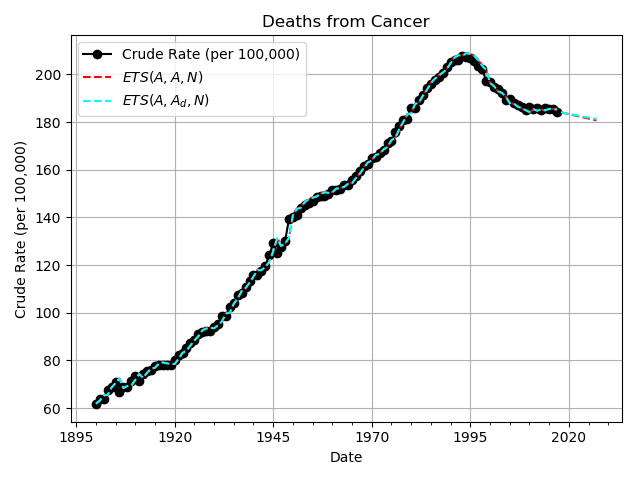
\includegraphics[width=0.5\textwidth]{results/US_ICD_LONGTERM_COMPARABLE_LEADING_Cancer_ets.png}
  \caption{Exponential smoothing functions $ETS(A,A*,N),\phi=0.98$ using Holt's linear trend method for \textit{Cancer} for the Longterm comparable leading causes of death for the United States}\label{fig:fig1}
\end{figure}

Scedasticity, forecast uncertainty, and cross-validation are not considered because it's not clear how to automate processing of such data to tune or choose models.

For each model, calculate AICc and choose the model $M(A(t_F))$ that has the lowest AICc.
For example, see Table \ref{table:choosem}:

\begin{table}[H]
  \centering
  \begin{tabular}{lcc}
    \toprule
      $R_i(D(A))$       & AICc            & Predicted       \\
    \midrule
      $\bm{ETS(A,A,N)}$ & \textbf{128.37} & \textbf{180.73} \\
      $ETS(A,A_d,N)$    & 128.83          & 181.29          \\
    \bottomrule
  \end{tabular}
  \caption{Example AICc values of $R_i(D(A))$ for \textit{Cancer} for the Longterm comparable leading causes of death for the United States}
  \label{table:choosem}
\end{table}

Use each $M(A(t_F))$'s predicted value (setting negative values to 0) and generate all of the relative $B(t_F)$ values along with any scale functions based on the models (e.g. scaling by the relative prediction derivatives using $S_3$).
For example, see Table \ref{table:btable}:

\begin{table}[H]
  \centering
  \begin{tabular}{lccc}
    \toprule
      Action  & $B(t_F)$ & $S_1$  & $S_3$  \\
    \midrule
      Name02  & 0.305    & 1      & 0.682  \\
      Name18  & 0.281    & 1      & 0.634  \\
      \ldots  & \ldots   & \ldots & \ldots \\
    \bottomrule
  \end{tabular}
  \caption{Example $B(t_F)$ values and model-based scale function values for the Longterm comparable leading causes of death for the United States}
  \label{table:btable}
\end{table}

Combine the table above with the manually calculated scale functions table (Table \ref{table:scaletable}) and any other calculated scale functions (e.g. $S_2(A_i)$) to create the final table with all scale function values.
For example, see Table \ref{table:btablewithall}:

\begin{table}[H]
  \centering
  \begin{tabular}{lccccc}
    \toprule
      Action  & $B(t_F)$ & $S_1$  & $S_2$  & $S_3$  & $S_4$  \\
    \midrule
      Name02  & 0.305    & 1      & 0.386  & 0.682  & 1      \\
      Name18  & 0.281    & 1      & 0.435  & 0.634  & 1      \\
      \ldots  & \ldots   & \ldots & \ldots & \ldots & \ldots \\
    \bottomrule
  \end{tabular}
  \caption{Example $B(t_F)$ values with all scale function values for the Longterm comparable leading causes of death for the United States}
  \label{table:btablewithall}
\end{table}

Calculate the product of each action's $B(t_F)$ and its scale function values to produce the final $Z(t_F)$ table and then sort by the values in descending order and choose the top $k$ actions.

This analysis is run on all mutually exclusive groupings of causes of death\footnote{See Appendix command \ref{cmdmodeledvbpus}.}:

\clearpage

\subsection{Results}

\subsubsection{Longterm comparable leading causes of death for the United States}

Top 5 MVBP results for the longterm comparable leading causes of death for the United States\footnote{See Appendix command \ref{cmdlongtermcomparable}.} in Table \ref{table:ztable1} and Figures \ref{fig:k1a}-\ref{fig:k1e}:

% US_ICD_LONGTERM_COMPARABLE_LEADING
\begin{table}[H]
  \centering
  \begin{tabular}{clc}
    \toprule
      $k$ & Action (Eliminate: \ldots) & $Z(t_F)$ \\
    \midrule
      1 &                      Heart disease & 0.080375 \\
      2 &                             Cancer & 0.077476 \\
      3 &       Chronic respiratory diseases & 0.034373 \\
      4 & Accidents excluding motor vehicles & 0.025423 \\
      5 &                           Diabetes & 0.014776 \\
    \bottomrule
  \end{tabular}
  \caption{$Z(t_F)$ table for the Longterm comparable leading causes of death for the United States}
  \label{table:ztable1}
\end{table}

\begin{figure}[H]
  \centering
  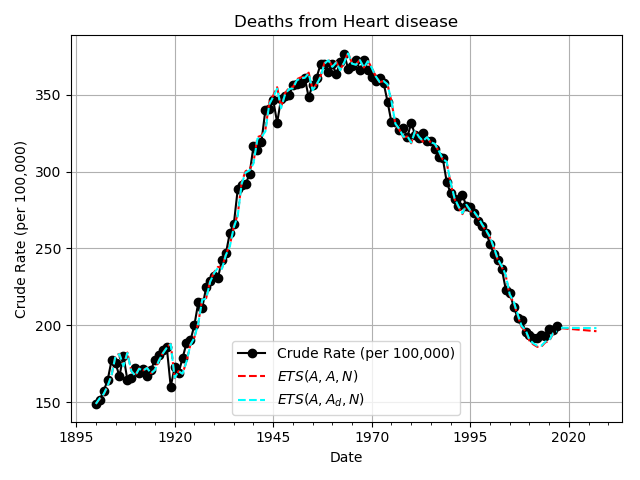
\includegraphics[width=0.5\textwidth]{results/US_ICD_LONGTERM_COMPARABLE_LEADING/Heart_disease_ets.png}
  \caption{First priority action from the Longterm comparable leading causes of death for the United States: \textit{Heart disease}}\label{fig:k1a}
\end{figure}

\begin{figure}[H]
  \centering
  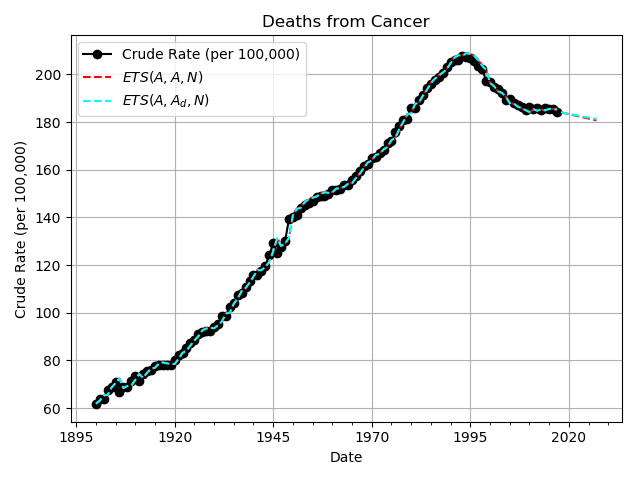
\includegraphics[width=0.5\textwidth]{results/US_ICD_LONGTERM_COMPARABLE_LEADING/Cancer_ets.png}
  \caption{Second priority action from the Longterm comparable leading causes of death for the United States: \textit{Cancer}}\label{fig:k1b}
\end{figure}

\begin{figure}[H]
  \centering
  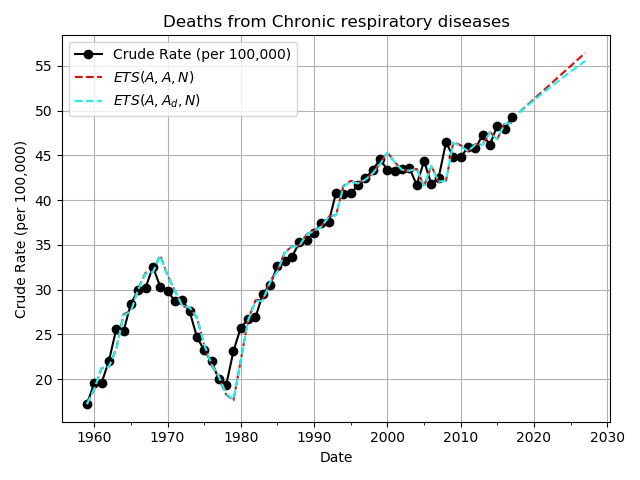
\includegraphics[width=0.5\textwidth]{results/US_ICD_LONGTERM_COMPARABLE_LEADING/Chronic_respiratory_diseases_ets.png}
  \caption{Third priority action from the Longterm comparable leading causes of death for the United States: \textit{Chronic respiratory diseases}}\label{fig:k1c}
\end{figure}

\begin{figure}[H]
  \centering
  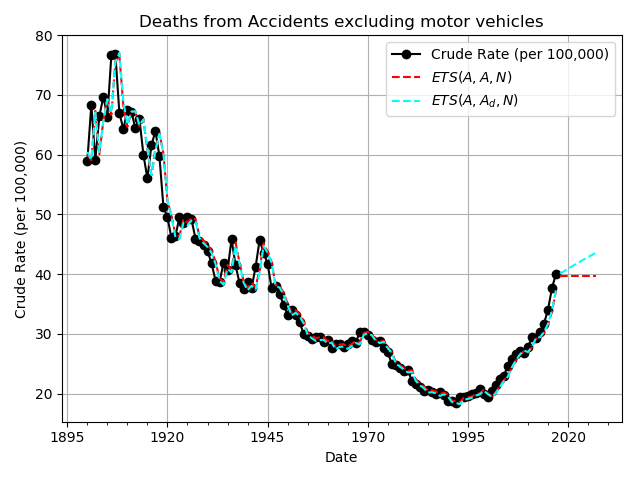
\includegraphics[width=0.5\textwidth]{results/US_ICD_LONGTERM_COMPARABLE_LEADING/Accidents_excluding_motor_vehicles_ets.png}
  \caption{Fourth priority action from the Longterm comparable leading causes of death for the United States: \textit{Accidents excluding motor vehicles}}\label{fig:k1d}
\end{figure}

\begin{figure}[H]
  \centering
  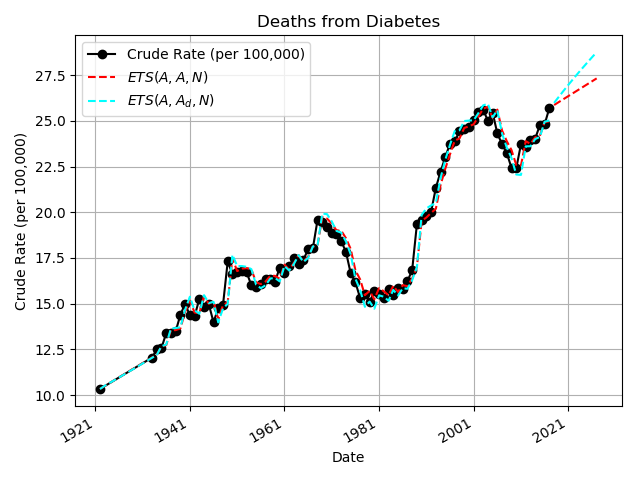
\includegraphics[width=0.5\textwidth]{results/US_ICD_LONGTERM_COMPARABLE_LEADING/Diabetes_ets.png}
  \caption{Fifth priority action from the Longterm comparable leading causes of death for the United States: \textit{Diabetes}}\label{fig:k1e}
\end{figure}

\clearpage

\subsubsection{ICD-9 and ICD-10 113 Cause List for the United States}

% US_ICD_113_SELECTED_CAUSES_LEAVES
Top 5 MVBP results for the ICD-9 and ICD-10 113 Cause List for the United States \citep{nbermortality,anderson2001comparability,icdcomparabilityratios,centers2017underlying}\textsuperscript{,}\footnote{\scriptsize{\url{ftp://ftp.cdc.gov/pub/Health_Statistics/NCHS/Datasets/Comparability/icd9_icd10/Comparability_Ratio_tables.xls}}}\textsuperscript{,}\footnote{\scriptsize{\url{https://wonder.cdc.gov/wonder/help/ucd.html\#ICD-10\%20113\%20Cause\%20List}}}\textsuperscript{,}\footnote{\scriptsize{\url{https://www.cdc.gov/nchs/data/dvs/Multiple_Cause_Record_Layout_2016.pdf}, page 19; The list actually has 118 mututally exclusive groups instead of 113.}} in Table \ref{table:ztable2} and Figures \ref{fig:k2a}-\ref{fig:k2e}:

\begin{table}[H]
  \centering
  \begin{tabular}{clc}
    \toprule
      $k$ & Action (Eliminate: \ldots) & $Z(t_F)$ \\
    \midrule
      1 &                      Nontransport accidents & 0.032929 \\
      2 &  \ldots poisoning \ldots noxious substances & 0.025236 \\
      3 &                     Ischemic heart diseases & 0.022342 \\
      4 &                    Cerebrovascular diseases & 0.015068 \\
      5 &    Other chronic lower respiratory diseases & 0.013543 \\
  \end{tabular}
  \caption{$Z(t_F)$ table for the ICD-9 and ICD-10 113 Cause List for the United States}
  \label{table:ztable2}
\end{table}

\begin{figure}[H]
  \centering
  \includegraphics[width=0.5\textwidth]{results/US_ICD_113_SELECTED_CAUSES_LEAVES/Nontransport_accidents_ets.png}
  \caption{First priority action from the ICD-9 and ICD-10 113 Cause List for the United States: \textit{Nontransport accidents}}\label{fig:k2a}
\end{figure}

\begin{figure}[H]
  \centering
  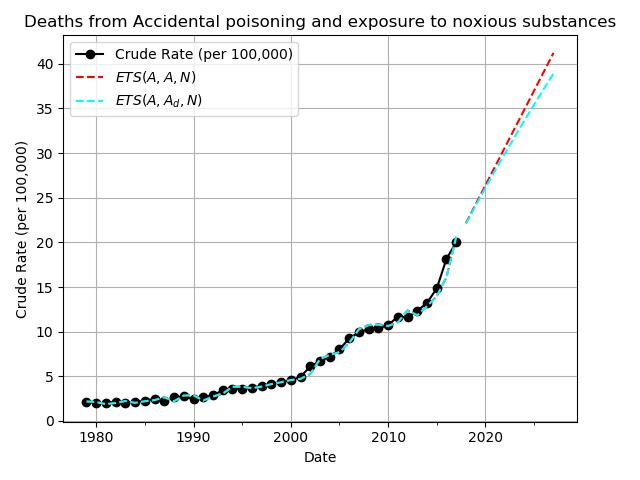
\includegraphics[width=0.5\textwidth]{results/US_ICD_113_SELECTED_CAUSES_LEAVES/Accidental_poisoning_and_exposure_to_noxious_substances_ets.png}
  \caption{Second priority action from the ICD-9 and ICD-10 113 Cause List for the United States: \textit{Accidental poisoning and exposure to noxious substances}}\label{fig:k2b}
\end{figure}

\begin{figure}[H]
  \centering
  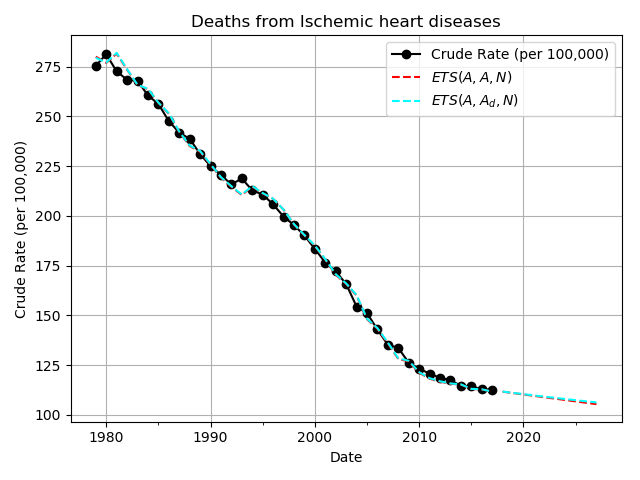
\includegraphics[width=0.5\textwidth]{results/US_ICD_113_SELECTED_CAUSES_LEAVES/Ischemic_heart_diseases_ets.png}
  \caption{Third priority action from the ICD-9 and ICD-10 113 Cause List for the United States: \textit{Ischemic heart diseases}}\label{fig:k2c}
\end{figure}

\begin{figure}[H]
  \centering
  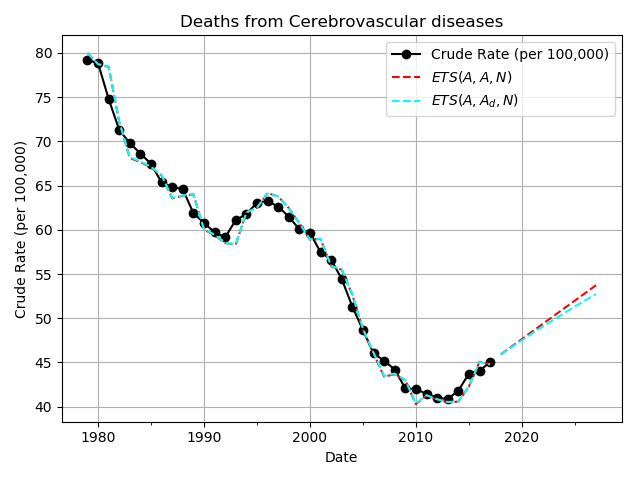
\includegraphics[width=0.5\textwidth]{results/US_ICD_113_SELECTED_CAUSES_LEAVES/Cerebrovascular_diseases_ets.png}
  \caption{Fourth priority action from the ICD-9 and ICD-10 113 Cause List for the United States: \textit{Cerebrovascular diseases}}\label{fig:k2d}
\end{figure}

\begin{figure}[H]
  \centering
  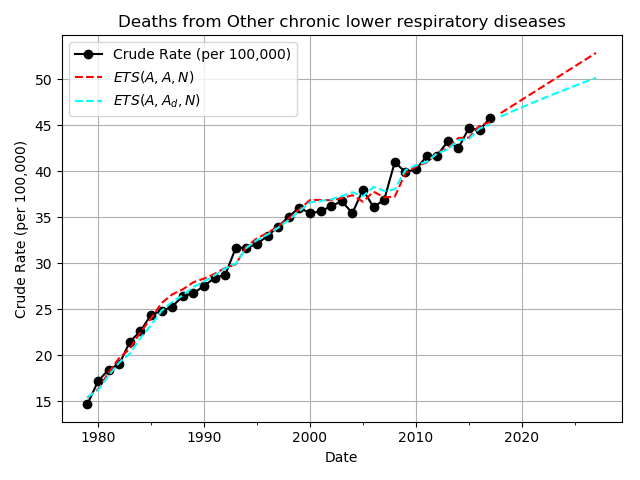
\includegraphics[width=0.5\textwidth]{results/US_ICD_113_SELECTED_CAUSES_LEAVES/Other_chronic_lower_respiratory_diseases_ets.png}
  \caption{Fifth priority action from the ICD-9 and ICD-10 113 Cause List for the United States: \textit{Other chronic lower respiratory diseases}}\label{fig:k2e}
\end{figure}

\clearpage

\subsubsection{ICD-9 and ICD-10 113 Cause List for the United States, including subtotals}

% US_ICD_113_SELECTED_CAUSES_ALL
Top 5 MVBP results for the ICD-9 and ICD-10 113 Cause List for the United States, including subtotals in Table \ref{table:ztable2} and Figures \ref{fig:k3a}-\ref{fig:k3e}:

\begin{table}[H]
  \centering
  \begin{tabular}{clc}
    \toprule
      $k$ & Action (Eliminate: \ldots) & $Z(t_F)$ \\
    \midrule
      1 &      Major cardiovascular diseases & 0.049639 \\
      2 &                  Diseases of heart & 0.031924 \\
      3 &                Malignant neoplasms & 0.019465 \\
      4 & Accidents (unintentional injuries) & 0.019337 \\
      5 &             Nontransport accidents & 0.014394 \\
  \end{tabular}
  \caption{$Z(t_F)$ table for the ICD-9 and ICD-10 113 Cause List for the United States, including subtotals}
  \label{table:ztable2}
\end{table}

\begin{figure}[H]
  \centering
  \includegraphics[width=0.5\textwidth]{results/US_ICD_113_SELECTED_CAUSES_ALL/Major_cardiovascular_diseases_ets.png}
  \caption{First priority action from the ICD-9 and ICD-10 113 Cause List for the United States, including subtotals: \textit{Major cardiovascular diseases}}\label{fig:k3a}
\end{figure}

\begin{figure}[H]
  \centering
  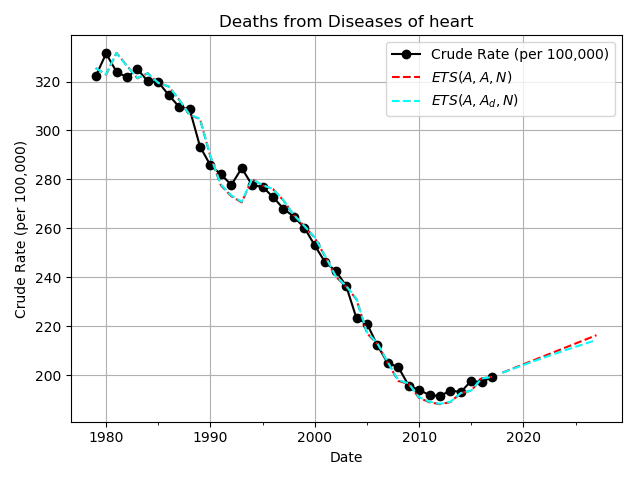
\includegraphics[width=0.5\textwidth]{results/US_ICD_113_SELECTED_CAUSES_ALL/Diseases_of_heart_ets.png}
  \caption{Second priority action from the ICD-9 and ICD-10 113 Cause List for the United States, including subtotals: \textit{Diseases of heart}}\label{fig:k3b}
\end{figure}

\begin{figure}[H]
  \centering
  \includegraphics[width=0.5\textwidth]{results/US_ICD_113_SELECTED_CAUSES_ALL/Malignant_neoplasms_ets.png}
  \caption{Third priority action from the ICD-9 and ICD-10 113 Cause List for the United States, including subtotals: \textit{Malignant neoplasms}}\label{fig:k3d}
\end{figure}

\begin{figure}[H]
  \centering
  \includegraphics[width=0.5\textwidth]{results/US_ICD_113_SELECTED_CAUSES_ALL/Accidents_unintentional_injuries_ets.png}
  \caption{Fourth priority action from the ICD-9 and ICD-10 113 Cause List for the United States, including subtotals: \textit{Accidents (unintentional injuries)}}\label{fig:k3e}
\end{figure}

\begin{figure}[H]
  \centering
  \includegraphics[width=0.5\textwidth]{results/US_ICD_113_SELECTED_CAUSES_ALL/Nontransport_accidents_ets.png}
  \caption{Fifth priority action from the ICD-9 and ICD-10 113 Cause List for the United States, including subtotals: \textit{Nontransport accidents}}\label{fig:k3c}
\end{figure}

\clearpage

\subsubsection{ICD-9 and ICD-10 113 Cause List for the United States with only top-level groupings}

% US_ICD_113_SELECTED_CAUSES_ROOTS
Top 5 MVBP results for the ICD-9 and ICD-10 113 Cause List for the United States with only top-level groupings in Table \ref{table:ztable3} and Figures \ref{fig:k4a}-\ref{fig:k4e}:

\begin{table}[H]
  \centering
  \begin{tabular}{clc}
    \toprule
      $k$ & Action (Eliminate: \ldots) & $Z(t_F)$ \\
    \midrule
      1 &      Major cardiovascular diseases & 0.131121 \\
      2 & Accidents (unintentional injuries) & 0.050850 \\
      3 &                Malignant neoplasms & 0.045513 \\
      4 & Chronic lower respiratory diseases & 0.017207 \\
      5 &                Alzheimer's disease & 0.012517 \\
    \bottomrule
  \end{tabular}
  \caption{$Z(t_F)$ table for the ICD-9 and ICD-10 113 Cause List for the United States with only top-level groupings}
  \label{table:ztable3}
\end{table}

\begin{figure}[H]
  \centering
  \includegraphics[width=0.5\textwidth]{results/US_ICD_113_SELECTED_CAUSES_ROOTS/Major_cardiovascular_diseases_ets.png}
  \caption{First priority action from the ICD-9 and ICD-10 113 Cause List for the United States with only top-level groupings: \textit{Major cardiovascular diseases}}\label{fig:k4a}
\end{figure}

\begin{figure}[H]
  \centering
  \includegraphics[width=0.5\textwidth]{results/US_ICD_113_SELECTED_CAUSES_ROOTS/Accidents_unintentional_injuries_ets.png}
  \caption{Second priority action from the ICD-9 and ICD-10 113 Cause List for the United States with only top-level groupings: \textit{Accidents (unintentional injuries)}}\label{fig:k4b}
\end{figure}

\begin{figure}[H]
  \centering
  \includegraphics[width=0.5\textwidth]{results/US_ICD_113_SELECTED_CAUSES_ROOTS/Malignant_neoplasms_ets.png}
  \caption{Third priority action from the ICD-9 and ICD-10 113 Cause List for the United States with only top-level groupings: \textit{Malignant neoplasms}}\label{fig:k4c}
\end{figure}

\begin{figure}[H]
  \centering
  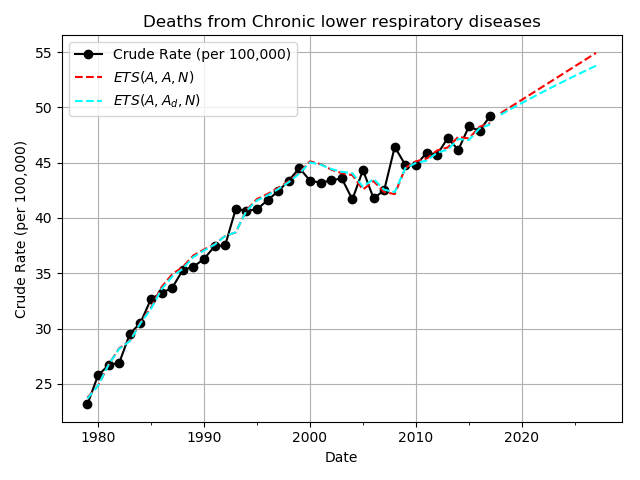
\includegraphics[width=0.5\textwidth]{results/US_ICD_113_SELECTED_CAUSES_ROOTS/Chronic_lower_respiratory_diseases_ets.png}
  \caption{Fourth priority action from the ICD-9 and ICD-10 113 Cause List for the United States with only top-level groupings: \textit{Chronic lower respiratory diseases}}\label{fig:k4d}
\end{figure}

\begin{figure}[H]
  \centering
  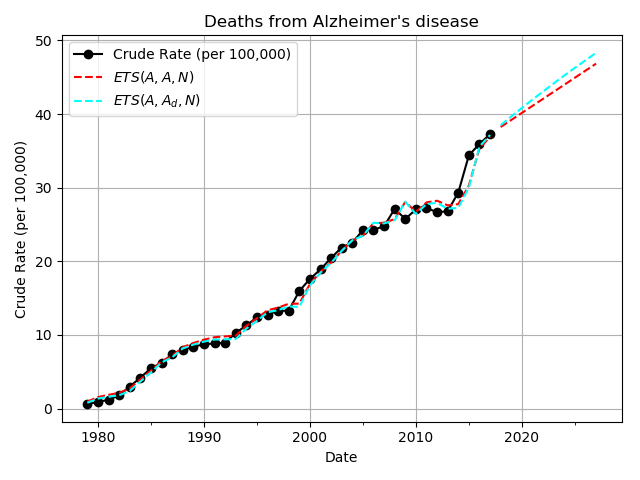
\includegraphics[width=0.5\textwidth]{results/US_ICD_113_SELECTED_CAUSES_ROOTS/Alzheimer_s_disease_ets.png}
  \caption{Fifth priority action from the ICD-9 and ICD-10 113 Cause List for the United States with only top-level groupings: \textit{Alzheimer's disease}}\label{fig:k4e}
\end{figure}

\clearpage

\subsubsection{ICD-10 Chapters for the United States}

% US_ICD10_CHAPTERS
Top 5 MVBP results for the ICD-10 Chapters for the United States \citep{centers2017underlying}\textsuperscript{,}\footnote{Group Results By \enquote{Year} And By \enquote{ICD Chapter}; Check \enquote{Export Results}; Uncheck \enquote{Show Totals}} in Table \ref{table:ztable5} and Figures \ref{fig:k5a}-\ref{fig:k5e}:

\begin{table}[H]
  \centering
  \begin{tabular}{clc}
    \toprule
      $k$ & Action (Eliminate: \ldots) & $Z(t_F)$ \\
    \midrule
      1 &         Diseases of the circulatory system & 0.101677 \\
      2 &        External causes of morbidity \ldots & 0.060121 \\
      3 &                                  Neoplasms & 0.039507 \\
      4 &             Diseases of the nervous system & 0.037175 \\
      5 &         Diseases of the respiratory system & 0.026494 \\
  \end{tabular}
  \caption{$Z(t_F)$ table for the ICD-10 Chapters for the United States}
  \label{table:ztable5}
\end{table}

\begin{figure}[H]
  \centering
  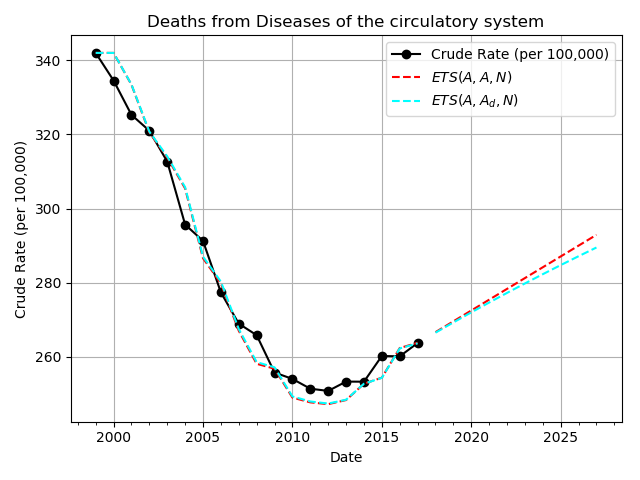
\includegraphics[width=0.5\textwidth]{results/US_ICD10_CHAPTERS/Diseases_of_the_circulatory_system_ets.png}
  \caption{First priority action from the ICD-10 Chapters for the United States: \textit{Diseases of the circulatory system}}\label{fig:k5a}
\end{figure}

\begin{figure}[H]
  \centering
  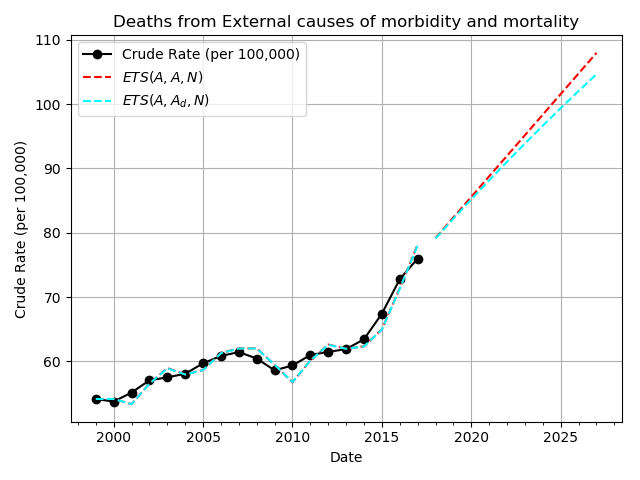
\includegraphics[width=0.5\textwidth]{results/US_ICD10_CHAPTERS/External_causes_of_morbidity_and_mortality_ets.png}
  \caption{Second priority action from the ICD-10 Chapters for the United States: \textit{External causes of morbidity and mortality}}\label{fig:k5b}
\end{figure}

\begin{figure}[H]
  \centering
  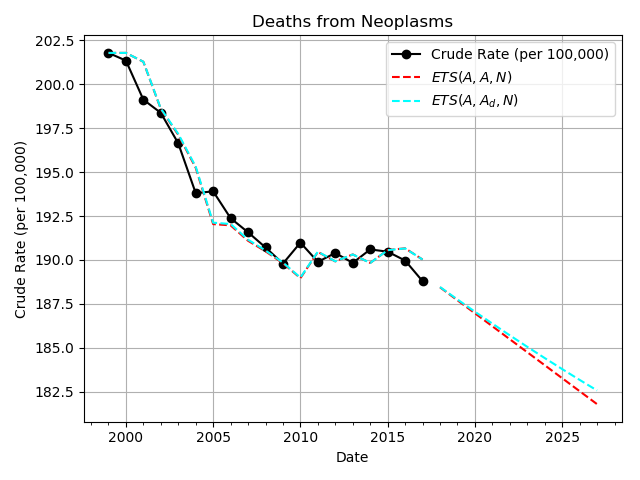
\includegraphics[width=0.5\textwidth]{results/US_ICD10_CHAPTERS/Neoplasms_ets.png}
  \caption{Third priority action from the ICD-10 Chapters for the United States: \textit{Neoplasms}}\label{fig:k5c}
\end{figure}

\begin{figure}[H]
  \centering
  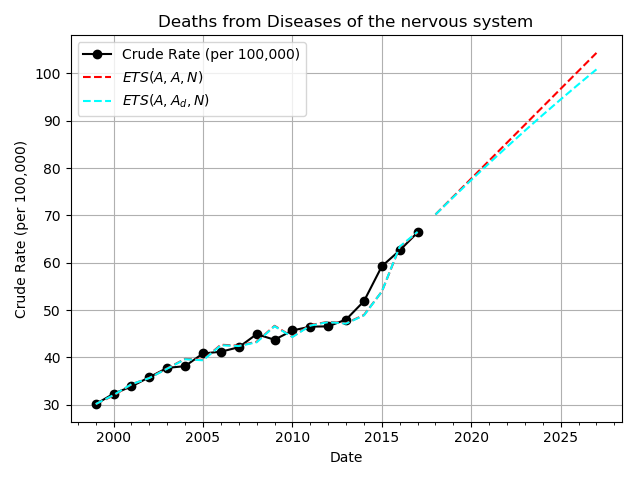
\includegraphics[width=0.5\textwidth]{results/US_ICD10_CHAPTERS/Diseases_of_the_nervous_system_ets.png}
  \caption{Fourth priority action from the ICD-10 Chapters for the United States: \textit{Diseases of the nervous system}}\label{fig:k5d}
\end{figure}

\begin{figure}[H]
  \centering
  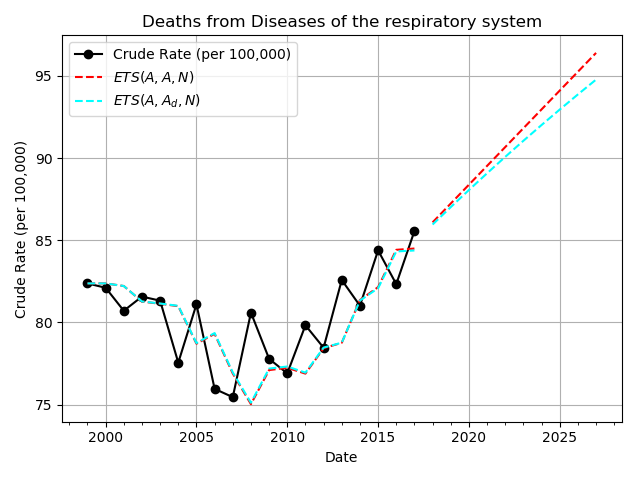
\includegraphics[width=0.5\textwidth]{results/US_ICD10_CHAPTERS/Diseases_of_the_respiratory_system_ets.png}
  \caption{Fifth priority action from the ICD-10 Chapters for the United States: \textit{Diseases of the respiratory system}}\label{fig:k5e}
\end{figure}

\clearpage

\subsubsection{ICD-10 Sub-Chapters for the United States}

% US_ICD10_SUB_CHAPTERS
Top 5 MVBP results for the ICD-10 Sub-Chapters for the United States \citep{centers2017underlying}\textsuperscript{,}\footnote{Group Results By \enquote{Year} And By \enquote{ICD Sub-Chapter}; Check \enquote{Export Results}; Uncheck \enquote{Show Totals}} in Table \ref{table:ztable6} and Figures \ref{fig:k6a}-\ref{fig:k6e}:

\begin{table}[H]
  \centering
  \begin{tabular}{clc}
    \toprule
      $k$ & Action (Eliminate: \ldots) & $Z(t_F)$ \\
    \midrule
      1 &                               Malignant neoplasms & 0.042786 \\
      2 &        Other external causes of accidental injury & 0.036444 \\
      3 &                      Other forms of heart disease & 0.023138 \\
      4 &                          Ischaemic heart diseases & 0.022449 \\
      5 &       Other \ldots diseases of the nervous system & 0.016669 \\
    \bottomrule
  \end{tabular}
  \caption{$Z(t_F)$ table for the ICD-10 Sub-Chapters for the United States}
  \label{table:ztable6}
\end{table}

\begin{figure}[H]
  \centering
  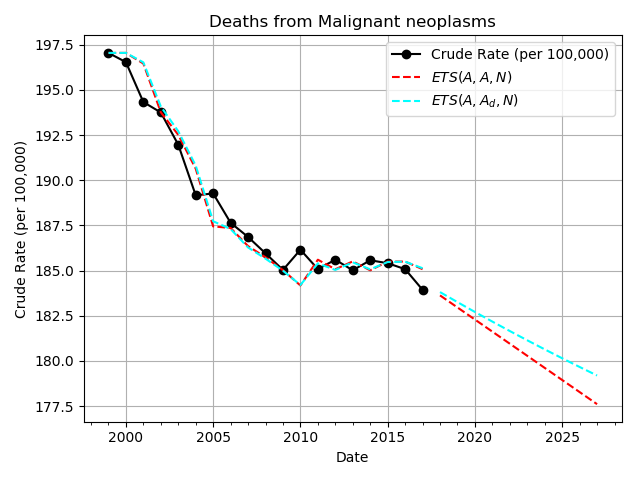
\includegraphics[width=0.5\textwidth]{results/US_ICD10_SUB_CHAPTERS/Malignant_neoplasms_ets.png}
  \caption{First priority action from the ICD-10 Sub-Chapters for the United States: \textit{Malignant neoplasms}}\label{fig:k6a}
\end{figure}
  
\begin{figure}[H]
  \centering
  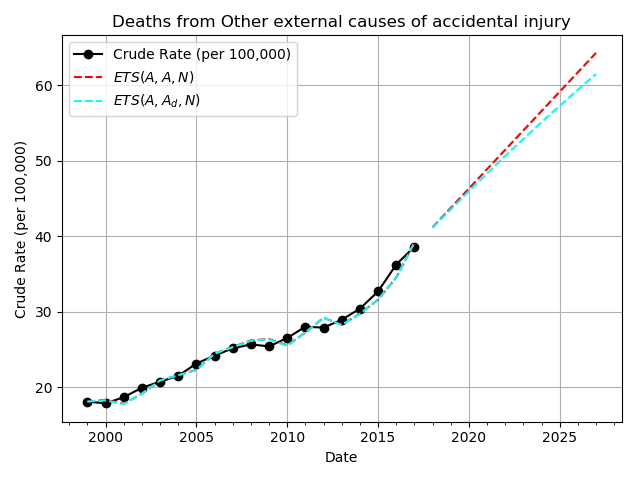
\includegraphics[width=0.5\textwidth]{results/US_ICD10_SUB_CHAPTERS/Other_external_causes_of_accidental_injury_ets.png}
  \caption{Second priority action from the ICD-10 Sub-Chapters for the United States: \textit{Other external causes of accidental injury}}\label{fig:k6b}
\end{figure}
  
\begin{figure}[H]
  \centering
  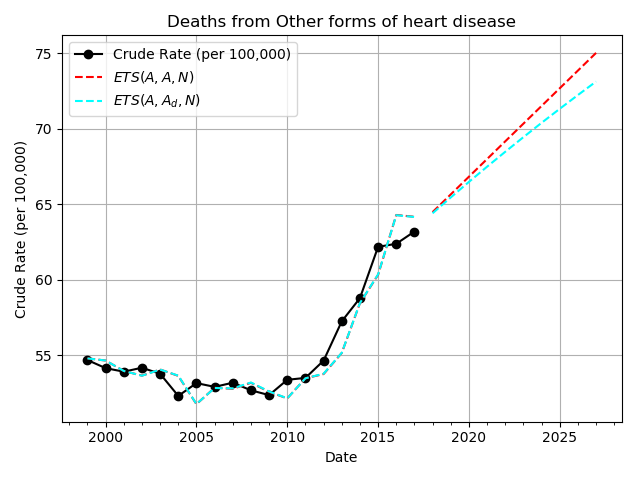
\includegraphics[width=0.5\textwidth]{results/US_ICD10_SUB_CHAPTERS/Other_forms_of_heart_disease_ets.png}
  \caption{Third priority action from the ICD-10 Sub-Chapters for the United States: \textit{Other forms of heart disease}}\label{fig:k6c}
\end{figure}
  
\begin{figure}[H]
  \centering
  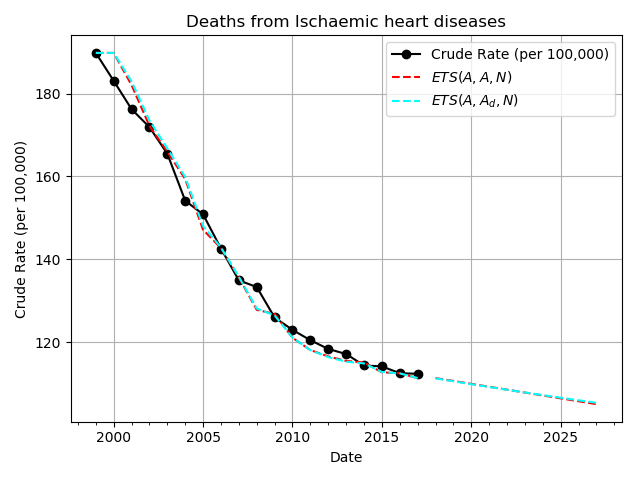
\includegraphics[width=0.5\textwidth]{results/US_ICD10_SUB_CHAPTERS/Ischaemic_heart_diseases_ets.png}
  \caption{Fourth priority action from the ICD-10 Sub-Chapters for the United States: \textit{Ischaemic heart diseases}}\label{fig:k6d}
\end{figure}
  
\begin{figure}[H]
  \centering
  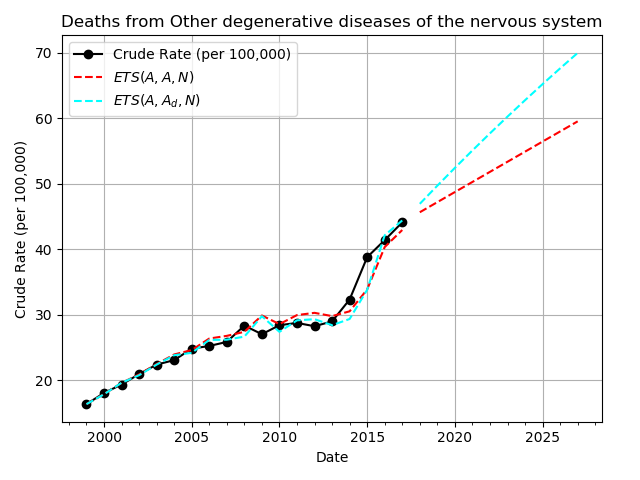
\includegraphics[width=0.5\textwidth]{results/US_ICD10_SUB_CHAPTERS/Other_degenerative_diseases_of_the_nervous_system_ets.png}
  \caption{Fifth priority action from the ICD-10 Sub-Chapters for the United States: \textit{Other degenerative diseases of the nervous system}}\label{fig:k6e}
\end{figure}
  
\clearpage

\subsubsection{Minimally grouped (5,264) causes of death for the United States}

% US_ICD10_MINIMALLY_GROUPED
Top 5 MVBP results for the minimally grouped (5,264) causes of death for the United States \citep{centers2017underlying}\textsuperscript{,}\footnote{Group Results By \enquote{Year} And By \enquote{Cause of death}; Check \enquote{Export Results}; Uncheck \enquote{Show Totals}}\textsuperscript{,}\footnote{Without $S_4$ due to the sheer number of causes.} in Table \ref{table:ztable7} and Figures \ref{fig:k7a}-\ref{fig:k7e}:

\begin{table}[H]
  \centering
  \begin{tabular}{clc}
    \toprule
      $k$ & Action (Eliminate: \ldots) & $Z(t_F)$ \\
    \midrule
      1 &                                Alzheimer disease, unspecified (G30.9) & 0.013730 \\
      2 &                                 Atherosclerotic heart disease (I25.1) & 0.012711 \\
      3 &                                     Accidental poisoning \ldots (X42) & 0.012563 \\
      4 &                         \ldots pulmonary disease, unspecified (J44.9) & 0.011704 \\
      5 &                              Cerebral infarction, unspecified (I63.9) & 0.007563 \\
    \bottomrule
  \end{tabular}
  \caption{$Z(t_F)$ table for the Minimally grouped (5,264) causes of death for the United States}
  \label{table:ztable7}
\end{table}

\begin{figure}[H]
  \centering
  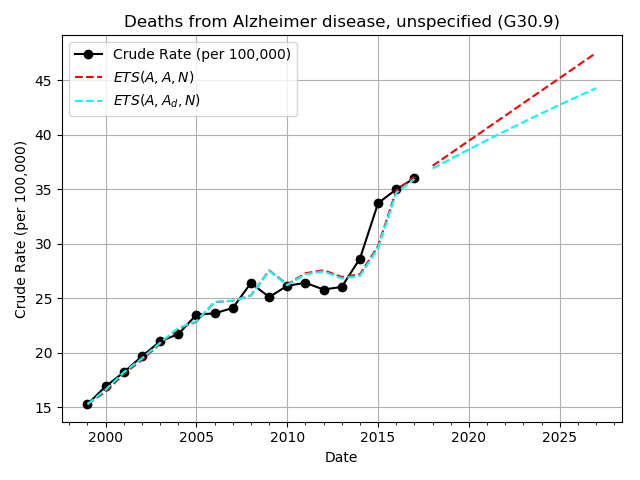
\includegraphics[width=0.5\textwidth]{results/US_ICD10_MINIMALLY_GROUPED/Alzheimer_disease_unspecified_G30_9_ets.png}
  \caption{First priority action from the Minimally grouped (5,264) causes of death for the United States: \textit{Alzheimer disease, unspecified (G30.9)}}\label{fig:k7a}
\end{figure}

\begin{figure}[H]
  \centering
  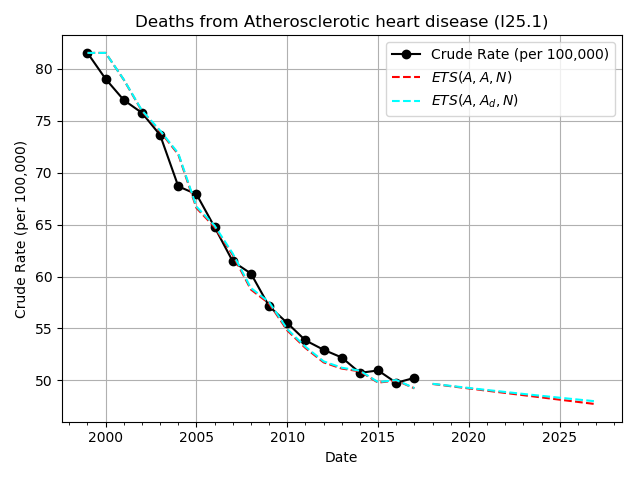
\includegraphics[width=0.5\textwidth]{results/US_ICD10_MINIMALLY_GROUPED/Atherosclerotic_heart_disease_I25_1_ets.png}
  \caption{Second priority action from the Minimally grouped (5,264) causes of death for the United States: \textit{Atherosclerotic heart disease (I25.1)}}\label{fig:k7b}
\end{figure}

\begin{figure}[H]
  \centering
  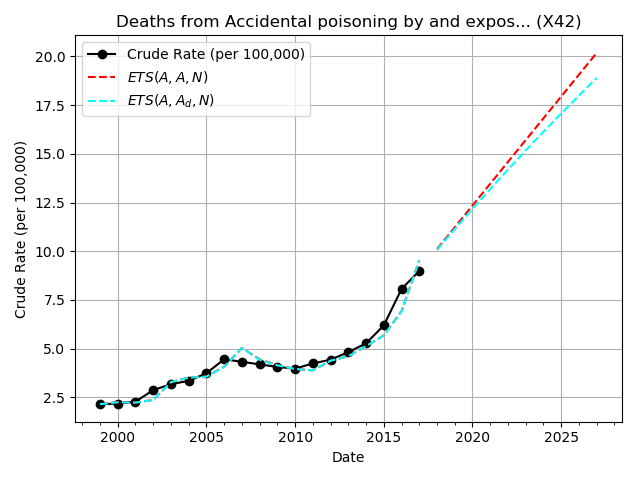
\includegraphics[width=0.5\textwidth]{results/US_ICD10_MINIMALLY_GROUPED/Accidental_poisoning_by_and_exposure_to_narcotics_and_psychodysleptics_hallucinogens_not_elsewhere_classified_X42_ets.png}
  \caption{Third priority action from the Minimally grouped (5,264) causes of death for the United States: \textit{Accidental poisoning by and exposure to narcotics and psychodysleptics [hallucinogens] not elsewhere classified (X42)}}\label{fig:k7c}
\end{figure}

\begin{figure}[H]
  \centering
  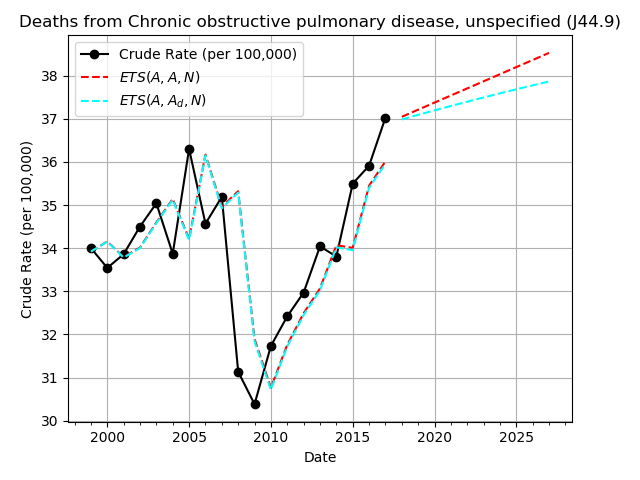
\includegraphics[width=0.5\textwidth]{results/US_ICD10_MINIMALLY_GROUPED/Chronic_obstructive_pulmonary_disease_unspecified_J44_9_ets.png}
  \caption{Fourth priority action from the Minimally grouped (5,264) causes of death for the United States: \textit{Chronic obstructive pulmonary disease, unspecified (J44.9)}}\label{fig:k7d}
\end{figure}

\begin{figure}[H]
  \centering
  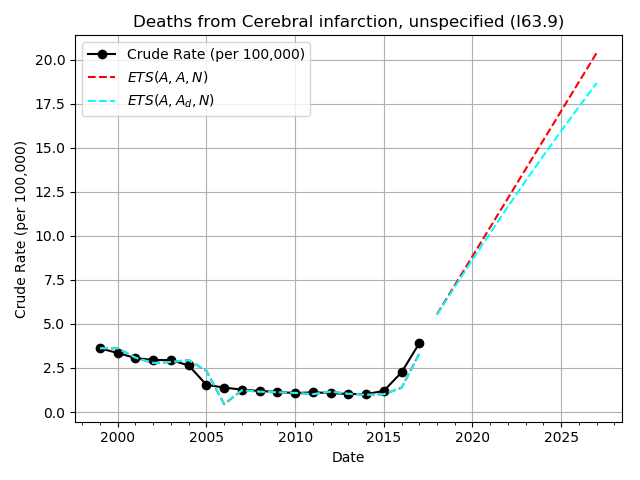
\includegraphics[width=0.5\textwidth]{results/US_ICD10_MINIMALLY_GROUPED/Cerebral_infarction_unspecified_I63_9_ets.png}
  \caption{Fifth priority action from the Minimally grouped (5,264) causes of death for the United States: \textit{Cerebral infarction, unspecified (I63.9)}}\label{fig:k7e}
\end{figure}

\clearpage

\subsubsection{Minimally grouped (11,316) causes of death for the World}

% WORLD_ICD10_MINIMALLY_GROUPED
Top 5 MVBP results for the minimally grouped (11,316) causes of death for the World \citep{whomortality,icd10vol1}\textsuperscript{,}\footnote{See Appendix command \ref{cmdmodeledvbpworld}.}\textsuperscript{,}\footnote{\label{no_s3}Without $S_3$ because comprehensive granular age data doesn't exist.}\textsuperscript{,}\footnote{Without $S_4$ due to the sheer number of causes.} in Table \ref{table:ztable8} and Figures \ref{fig:k8a}-\ref{fig:k8e}:

\begin{table}[H]
  \centering
  \begin{tabular}{clc}
    \toprule
      $k$ & Action (Eliminate: \ldots) & $Z(t_F)$ \\
    \midrule
      1 & \ldots neoplasm of bronchus \ldots (C34.9) & 0.026866 \\
      2 &                 Unspecified dementia (F03) & 0.024561 \\
      3 & Acute myocardial infarction \ldots (I21.9) & 0.022585 \\
      4 &             Other ill-defined \ldots (R99) & 0.019871 \\
      5 &         Heart failure, unspecified (I50.9) & 0.018749 \\
    \bottomrule
  \end{tabular}
  \caption{$Z(t_F)$ table for the Minimally grouped (11,316) causes of death for the World}
  \label{table:ztable8}
\end{table}

\begin{figure}[H]
  \centering
  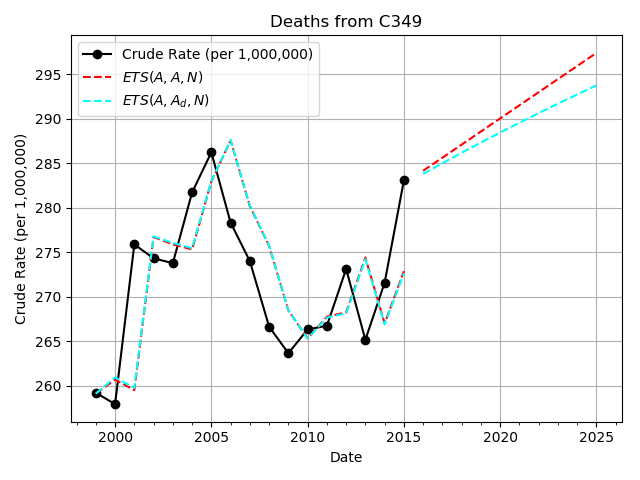
\includegraphics[width=0.5\textwidth]{results/WORLD_ICD10_MINIMALLY_GROUPED/C349_ets.png}
  \caption{First priority action from the Minimally grouped (11,316) causes of death for the World: \textit{Malignant neoplasm of bronchus and lung, unspecified (C34.9)}}\label{fig:k8a}
\end{figure}

\begin{figure}[H]
  \centering
  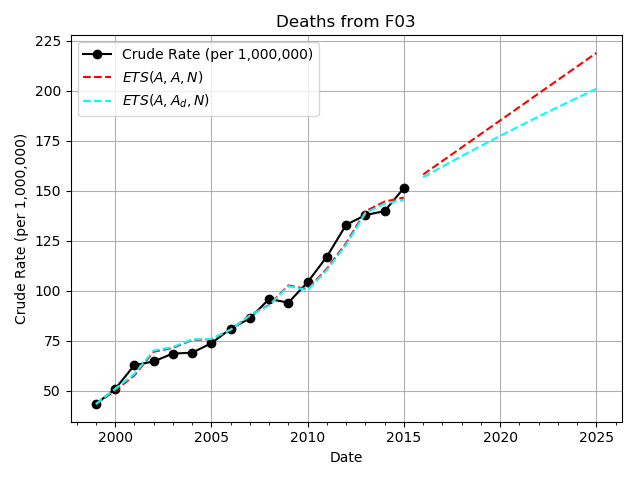
\includegraphics[width=0.5\textwidth]{results/WORLD_ICD10_MINIMALLY_GROUPED/F03_ets.png}
  \caption{Second priority action from the Minimally grouped (11,316) causes of death for the World: \textit{Unspecified dementia (F03)}}\label{fig:k8b}
\end{figure}

\begin{figure}[H]
  \centering
  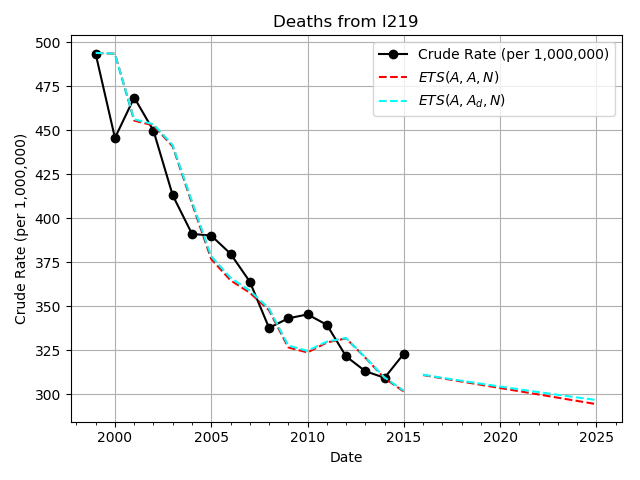
\includegraphics[width=0.5\textwidth]{results/WORLD_ICD10_MINIMALLY_GROUPED/I219_ets.png}
  \caption{Third priority action from the Minimally grouped (11,316) causes of death for the World: \textit{Acute myocardial infarction, unspecified (I21.9)}}\label{fig:k8c}
\end{figure}

\begin{figure}[H]
  \centering
  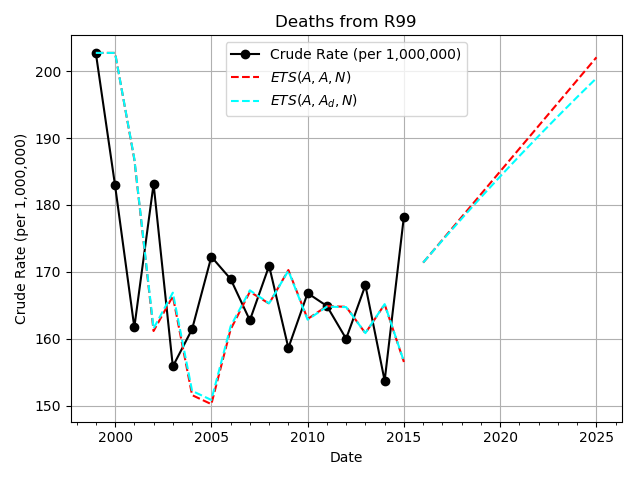
\includegraphics[width=0.5\textwidth]{results/WORLD_ICD10_MINIMALLY_GROUPED/R99_ets.png}
  \caption{Fourth priority action from the Minimally grouped (11,316) causes of death for the World: \textit{Other ill-defined and unspecified causes of mortality (R99)}}\label{fig:k8d}
\end{figure}

\begin{figure}[H]
  \centering
  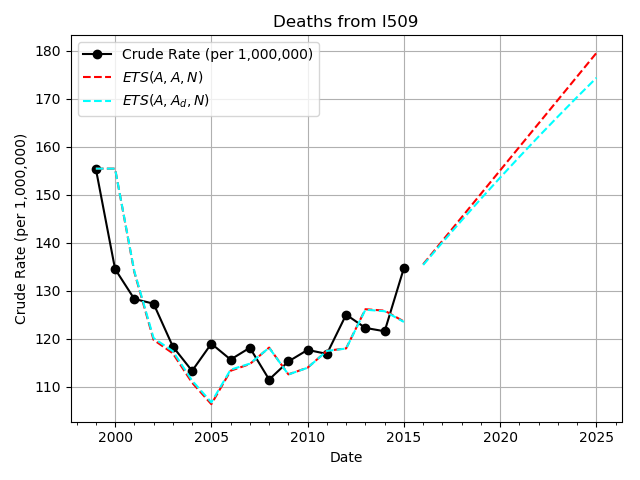
\includegraphics[width=0.5\textwidth]{results/WORLD_ICD10_MINIMALLY_GROUPED/I509_ets.png}
  \caption{Fifth priority action from the Minimally grouped (11,316) causes of death for the World: \textit{Heart failure, unspecified (I50.9)}}\label{fig:k8e}
\end{figure}

\clearpage

\subsubsection{ICD-10 Chapters for the World, including subtotals}

% WORLD_ICD10_CHAPTERS_ALL
Top 5 MVBP results for the ICD-10 Chapters for the World, including subtotals \citep{whomortality}\textsuperscript{,}\footnote{See footnote \ref{no_s3}.} in Table \ref{table:ztable9} and Figures \ref{fig:k9a}-\ref{fig:k9e}:

\begin{table}[H]
  \centering
  \begin{tabular}{clc}
    \toprule
      $k$ & Action (Eliminate: \ldots) & $Z(t_F)$ \\
    \midrule
      1 &          \ldots circulatory system (I00-I99) & 0.160800 \\
      2 &                          Neoplasms (C00-D48) & 0.097424 \\
      3 &                Malignant neoplasms (C00-C97) & 0.092250 \\
      4 &          \ldots respiratory system (J00-J99) & 0.046399 \\
      5 &           Ischaemic heart diseases (I20-I25) & 0.034819 \\
    \bottomrule
  \end{tabular}
  \caption{$Z(t_F)$ table for the ICD-10 Chapters for the World, including subtotals}
  \label{table:ztable9}
\end{table}

\begin{figure}[H]
  \centering
  \includegraphics[width=0.5\textwidth]{results/WORLD_ICD10_CHAPTERS_ALL/Diseases_of_the_circulatory_system_I00-I99_ets.png}
  \caption{First priority action from the ICD-10 Chapters for the World, including subtotals: \textit{Diseases of the circulatory system (I00-I99)}}\label{fig:k9a}
\end{figure}

\begin{figure}[H]
  \centering
  \includegraphics[width=0.5\textwidth]{results/WORLD_ICD10_CHAPTERS_ALL/Neoplasms_C00-D48_ets.png}
  \caption{Second priority action from the ICD-10 Chapters for the World, including subtotals: \textit{Neoplasms (C00-D48)}}\label{fig:k9b}
\end{figure}

\begin{figure}[H]
  \centering
  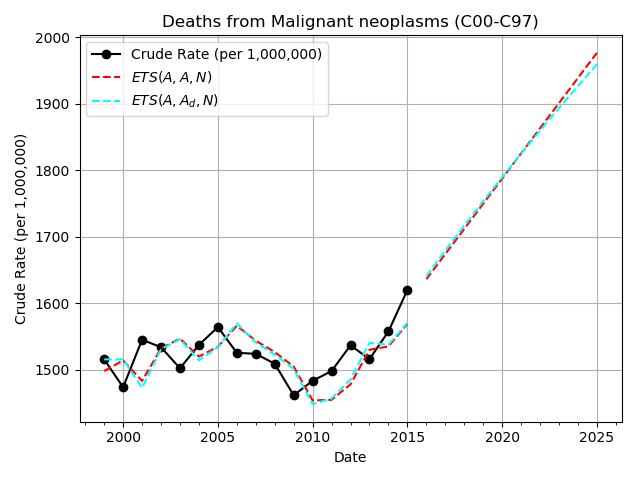
\includegraphics[width=0.5\textwidth]{results/WORLD_ICD10_CHAPTERS_ALL/Malignant_neoplasms_C00-C97_ets.png}
  \caption{Third priority action from the ICD-10 Chapters for the World, including subtotals: \textit{Malignant neoplasms (C00-C97)}}\label{fig:k9c}
\end{figure}

\begin{figure}[H]
  \centering
  \includegraphics[width=0.5\textwidth]{results/WORLD_ICD10_CHAPTERS_ALL/Diseases_of_the_respiratory_system_J00-J99_ets.png}
  \caption{Fourth priority action from the ICD-10 Chapters for the World, including subtotals: \textit{Diseases of the respiratory system (J00-J99)}}\label{fig:k9d}
\end{figure}

\begin{figure}[H]
  \centering
  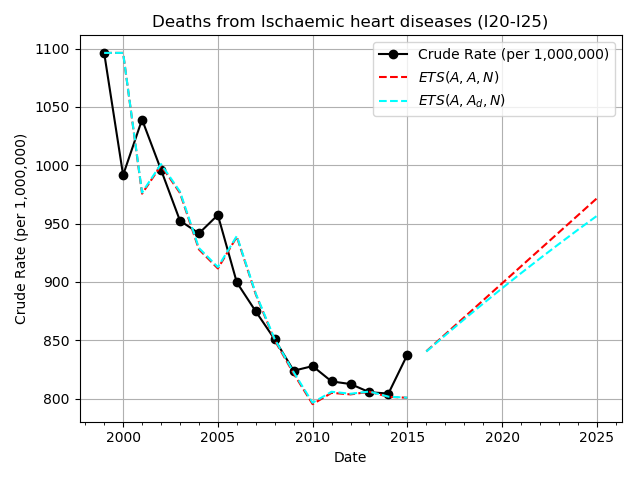
\includegraphics[width=0.5\textwidth]{results/WORLD_ICD10_CHAPTERS_ALL/Ischaemic_heart_diseases_I20-I25_ets.png}
  \caption{Fifth priority action from the ICD-10 Chapters for the World, including subtotals: \textit{Ischaemic heart diseases (I20-I25)}}\label{fig:k9e}
\end{figure}

\clearpage

\subsubsection{ICD-10 Chapters for the World with only top-level groupings}

% WORLD_ICD10_CHAPTER_ROOTS
Top 5 MVBP results for the ICD-10 Chapters for the World with only top-level groupings \citep{whomortality}\textsuperscript{,}\footnote{See footnote \ref{no_s3}.} in Table \ref{table:ztable10} and Figures \ref{fig:k10a}-\ref{fig:k10e}:

\begin{table}[H]
  \centering
  \begin{tabular}{clc}
    \toprule
      $k$ & Action (Eliminate: \ldots) & $Z(t_F)$ \\
    \midrule
      1 &         \ldots circulatory system (I00-I99) & 0.321104 \\
      2 &                         Neoplasms (C00-D48) & 0.194456 \\
      3 &         \ldots respiratory system (J00-J99) & 0.092581 \\
      4 &             \ldots nervous system (G00-G99) & 0.043816 \\
      5 &            External causes \ldots (V01-Y98) & 0.032951 \\
    \bottomrule
  \end{tabular}
  \caption{$Z(t_F)$ table for the ICD-10 Chapters for the World with only top-level groupings}
  \label{table:ztable10}
\end{table}

\begin{figure}[H]
  \centering
  \includegraphics[width=0.5\textwidth]{results/WORLD_ICD10_CHAPTER_ROOTS/Diseases_of_the_circulatory_system_I00-I99_ets.png}
  \caption{First priority action from the ICD-10 Chapters for the World with only top-level groupings: \textit{Diseases of the circulatory system (I00-I99)}}\label{fig:k10a}
\end{figure}

\begin{figure}[H]
  \centering
  \includegraphics[width=0.5\textwidth]{results/WORLD_ICD10_CHAPTER_ROOTS/Neoplasms_C00-D48_ets.png}
  \caption{Second priority action from the ICD-10 Chapters for the World with only top-level groupings: \textit{Neoplasms (C00-D48)}}\label{fig:k10b}
\end{figure}

\begin{figure}[H]
  \centering
  \includegraphics[width=0.5\textwidth]{results/WORLD_ICD10_CHAPTER_ROOTS/Diseases_of_the_respiratory_system_J00-J99_ets.png}
  \caption{Third priority action from the ICD-10 Chapters for the World with only top-level groupings: \textit{Diseases of the respiratory system (J00-J99)}}\label{fig:k10c}
\end{figure}

\begin{figure}[H]
  \centering
  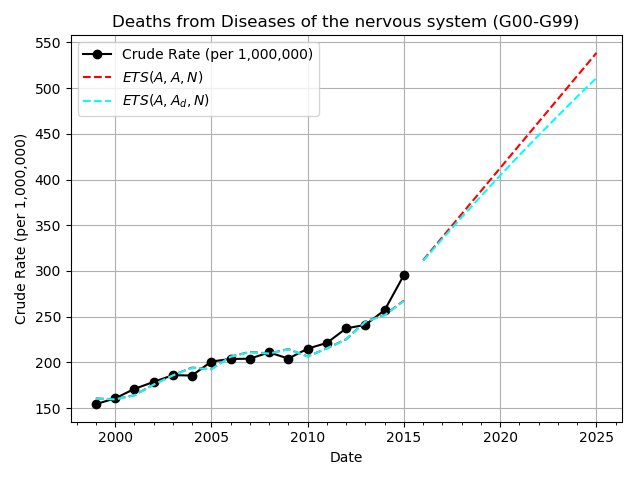
\includegraphics[width=0.5\textwidth]{results/WORLD_ICD10_CHAPTER_ROOTS/Diseases_of_the_nervous_system_G00-G99_ets.png}
  \caption{Fourth priority action from the ICD-10 Chapters for the World with only top-level groupings: \textit{Diseases of the nervous system (G00-G99)}}\label{fig:k10d}
\end{figure}

\begin{figure}[H]
  \centering
  \includegraphics[width=0.5\textwidth]{results/WORLD_ICD10_CHAPTER_ROOTS/External_causes_of_morbidity_and_mortality_V01-Y98_ets.png}
  \caption{Fifth priority action from the ICD-10 Chapters for the World with only top-level groupings: \textit{External causes of morbidity and mortality (V01-Y98)}}\label{fig:k10e}
\end{figure}

\clearpage

\subsubsection{ICD-10 Sub-Chapters for the World}

% WORLD_ICD10_SUB_CHAPTERS
Top 5 MVBP results for the ICD-10 Sub-Chapters for the World \citep{whomortality}\textsuperscript{,}\footnote{See footnote \ref{no_s3}.} in Table \ref{table:ztable11} and Figures \ref{fig:k11a}-\ref{fig:k11e}:

\begin{table}[H]
  \centering
  \begin{tabular}{clc}
    \toprule
      $k$ & Action (Eliminate: \ldots) & $Z(t_F)$ \\
    \midrule
      1 &                Malignant neoplasms (C00-C97) & 0.216971 \\
      2 &           Ischaemic heart diseases (I20-I25) & 0.076670 \\
      3 &       Other forms of heart disease (I30-I52) & 0.038095 \\
      4 &            Influenza and pneumonia (J09-J18) & 0.032015 \\
      5 &        \ldots respiratory diseases (J40-J47) & 0.031105 \\
    \bottomrule
  \end{tabular}
  \caption{$Z(t_F)$ table for the ICD-10 Sub-Chapters for the World}
  \label{table:ztable11}
\end{table}

\begin{figure}[H]
  \centering
  \includegraphics[width=0.5\textwidth]{results/WORLD_ICD10_SUB_CHAPTERS/Malignant_neoplasms_C00-C97_ets.png}
  \caption{First priority action from the ICD-10 Sub-Chapters for the World: \textit{Malignant neoplasms (C00-C97)}}\label{fig:k11a}
\end{figure}

\begin{figure}[H]
  \centering
  \includegraphics[width=0.5\textwidth]{results/WORLD_ICD10_SUB_CHAPTERS/Ischaemic_heart_diseases_I20-I25_ets.png}
  \caption{Second priority action from the ICD-10 Sub-Chapters for the World: \textit{Ischaemic heart diseases (I20-I25)}}\label{fig:k11b}
\end{figure}

\begin{figure}[H]
  \centering
  \includegraphics[width=0.5\textwidth]{results/WORLD_ICD10_SUB_CHAPTERS/Other_forms_of_heart_disease_I30-I52_ets.png}
  \caption{Third priority action from the ICD-10 Sub-Chapters for the World: \textit{Other forms of heart disease (I30-I52)}}\label{fig:k11c}
\end{figure}

\begin{figure}[H]
  \centering
  \includegraphics[width=0.5\textwidth]{results/WORLD_ICD10_SUB_CHAPTERS/Influenza_and_pneumonia_J09-J18_ets.png}
  \caption{Fourth priority action from the ICD-10 Sub-Chapters for the World: \textit{Influenza and pneumonia (J09-J18)}}\label{fig:k11d}
\end{figure}

\begin{figure}[H]
  \centering
  \includegraphics[width=0.5\textwidth]{results/WORLD_ICD10_SUB_CHAPTERS/Chronic_lower_respiratory_diseases_J40-J47_ets.png}
  \caption{Fifth priority action from the ICD-10 Sub-Chapters for the World: \textit{Chronic lower respiratory diseases (J40-J47)}}\label{fig:k11e}
\end{figure}

\clearpage

\subsubsection{Sub-selection}

Further sub-selection may be done by filtering by ICD codes\citep{icd10vol1}\textsuperscript{,}\footnote{See Appendix command \ref{cmdfilter}.}. For example, the top 5 MVBP results for the minimally grouped causes of death for the United States for heart diseases (codes I00-I99) in Table \ref{table:ztable12} and Figures \ref{fig:k12a}-\ref{fig:k12e}:

\begin{table}[H]
  \centering
  \begin{tabular}{clc}
    \toprule
      $k$ & Action (Eliminate: \ldots) & $Z(t_F)$ \\
    \midrule
      1 &        Atherosclerotic heart disease (I25.1) & 0.037527 \\
      2 & Atherosclerotic cardiovascular\ldots (I25.0) & 0.022493 \\
      3 &     Cerebral infarction, unspecified (I63.9) & 0.022395 \\
      4 &             Congestive heart failure (I50.0) & 0.015612 \\
      5 &    Hypertensive heart disease \ldots (I11.9) & 0.012890 \\
    \bottomrule
  \end{tabular}
  \caption{$Z(t_F)$ table for the minimally grouped causes of death for the United States for heart diseases (codes I00-I99)}
  \label{table:ztable12}
\end{table}

\begin{figure}[H]
  \centering
  \includegraphics[width=0.5\textwidth]{results/US_ICD10_MINIMALLY_GROUPED/Atherosclerotic_heart_disease_I25_1_ets.png}
  \caption{First priority action from the ICD-10 Sub-Chapters for the World: \textit{Atherosclerotic heart disease (I25.1)}}\label{fig:k12a}
\end{figure}

\begin{figure}[H]
  \centering
  \includegraphics[width=0.5\textwidth]{results/US_ICD10_MINIMALLY_GROUPED/Atherosclerotic_cardiovascular_disease_so_described_I25_0_ets.png}
  \caption{Second priority action from the ICD-10 Sub-Chapters for the World: \textit{Atherosclerotic cardiovascular disease, so described (I25.0)}}\label{fig:k12b}
\end{figure}

\begin{figure}[H]
  \centering
  \includegraphics[width=0.5\textwidth]{results/US_ICD10_MINIMALLY_GROUPED/Cerebral_infarction_unspecified_I63_9_ets.png}
  \caption{Third priority action from the ICD-10 Sub-Chapters for the World: \textit{Cerebral infarction, unspecified (I63.9)}}\label{fig:k12c}
\end{figure}

\begin{figure}[H]
  \centering
  \includegraphics[width=0.5\textwidth]{results/US_ICD10_MINIMALLY_GROUPED/Congestive_heart_failure_I50_0_ets.png}
  \caption{Fourth priority action from the ICD-10 Sub-Chapters for the World: \textit{Congestive heart failure (I50.0)}}\label{fig:k12d}
\end{figure}

\begin{figure}[H]
  \centering
  \includegraphics[width=0.5\textwidth]{results/US_ICD10_MINIMALLY_GROUPED/Hypertensive_heart_disease_without_congestive_heart_failure_I11_9_ets.png}
  \caption{Fifth priority action from the ICD-10 Sub-Chapters for the World: \textit{Hypertensive heart disease without (congestive) heart failure (I11.9)}}\label{fig:k12e}
\end{figure}

\clearpage

\section{Discussion}

This article proposes a method called value based prioritization which uses value theory to establish a goal and the set of known actions to accomplish said goal.
Each action is relatively ranked based on some quantitative measurement(s) as called for by the same value theory.
This ranking is transformed by a set of functions which scale up and down each action's relative score based on other relevant measurements and subjective opinions.
The resulting list provides a prioritized relative ranking of actions that should be pursued in a particular order.
Given that it may take significant time to ramp up and execute actions, modeled value based prioritization forecasts estimated relative rankings into the future to try to anticipate relative rankings by the time ramping up is complete.
In essence, value based prioritization is a method to triage the proper actions to take given limited time and resources.

This method is applied to the example of choosing meaningful work using an example value system based on the goal to reduce human suffering.
The method is sensitive to the choice of values and there are many ways to measure and scale the resulting relative rankings.
Even with pretty clear measurements such as death, which is a binary and straightforward metric, there are endless questions about data quality (\enquote{Garbage In, Garbage Out}), how to define the underlying cause of death, which data sets to use (\enquote{e.g. would world death rates significantly change if political conditions changed?}), etc.
Groupings of deaths introduce another dimension to evaluation: it's not clear how to relatively evaluate different groupings of deaths.
Finally, there is a significant risk of missing actions that don't neatly categorize into measurable quantities.
In short, there is no obvious way around certain philosophical questions, definitions, and evaluations.

Despite these shortcomings, alternative approaches are less quantitative, less explicit, and thus more difficult to evaluate and improve; and, more difficult to continuously evaluate progress on without such clear metrics. Further research and experience may help accumulate a database of value-metric mappings and scale functions that may be combined by people in different ways to help them prioritize actions such as finding meaningful work.

% Column break before the Bibliography.
%\vfill\eject

% https://tex.stackexchange.com/questions/329/how-to-change-font-size-for-bibliography
%{\footnotesize
\bibliography{value_based_prioritization}
%}

% Page break before the Appendix.
\newpage
\clearpage

\section{Appendix}

Notes on Section \ref{section-example}:

\begin{enumerate}
  \item \label{generateuslongterm} To generate the longterm comparable leading causes of death for the United States:
    \begin{enumerate}
      \item Generate data from 1959 for all long-term, comparable, leading causes of death\footnote{\scriptsize{\url{https://www.cdc.gov/nchs/data/dvs/lead1900_98.pdf}}}:
      
            \texttt{python3 -m vbp.run prepare\char`_data UCODUnitedStates}

      \item Rows 1900:1957 and the sheet \enquote{Comparability Ratios} in comparable\_ucod\_estimates.xlsx were manually input from \url{https://www.cdc.gov/nchs/data/dvs/lead1900_98.pdf}.
      \item Open comparable\_data\_since\_1959.xlsx and copy rows 1959:Present.
      \item Open comparable\_ucod\_estimates.xlsx and paste on top starting at 1959.
      \item Process comparable\_ucod\_estimates.xlsx with its \enquote{Comparability Ratios} sheet to generate comparable\_ucod\_estimates\_ratios\_applied.xlsx:
      
            \texttt{python3 -m vbp.run prepare\char`_data UCODUnitedStates --comparable-ratios}

    \end{enumerate}
  \item Age adjustment\footnote{\scriptsize{\url{https://seer.cancer.gov/seerstat/tutorials/aarates/definition.html}}} is not performed on crude rates because the goal of the example is to predict future \textit{relative} total death rates which already implicitly takes into account population age changes over time.
  \item The WHO Mortality Database population and death statistics are quite incomplete, reporting only about $\frac{1}{3}$ of the world population and about $\frac{1}{3}$ of world deaths:
    \begin{figure}[H]
      \centering
      \includegraphics[width=0.5\textwidth]{results/who_mortality_db_population_deaths.png}
      \caption{WHO Mortality Database: Reported Population and Deaths}
    \end{figure}
  \item \label{mathersquote} \enquote{There is a substantial literature on the projection or forecasting of all-cause mortality rates and mortality rates for specific diseases. The methods used fall into two broad groups. First are those methods based on time-series analysis of historical trends in mortality rates. These \enquote{aggregate models,} whether for all-cause mortality or for specific causes, use the previous trend of the variable of interest as the basis for predicting its future value. By their data requirements, such methods are generally limited to high-income countries with good death registration data [...]. Second are the \enquote{structural models,} which are based on relationships between mortality and a set of independent variables, and are necessarily projections of those independent variables. To the extent that the structural model identifies the important components — and the relationships among them — of the \enquote{system} that determines the variable of interest, they offer the potential for more robust predictions. When the underlying system is complex and sensitive to one or more of its components, a shift in some of the system variables can introduce large changes in the outcome that may be missed by extrapolation (such as the discovery of antibiotics and infectious disease trends or the change in tuberculosis mortality after the HIV epidemic). Aggregate models, in contrast, require considerably less knowledge of the system components and the relationships among them. These models can therefore provide more reliable estimates when such information is not available, especially when the system is not very sensitive to its inputs in time intervals that are in the order of the prediction time.} \citep{mathers2006projections}
  \item \enquote{Substantial research remains to develop robust and unbiased methods for measuring trends in case fatality rates, survival times, and disability due to specific causes, let alone collecting such data across all regions of the world. Despite these uncertainties, projections provide a useful perspective on population health trends and health policies, provided that they are interpreted with a degree of caution. Projections enable us to appreciate better the implications for health and health policy of currently observed trends, and the likely impact of fairly certain future trends, such as the ageing of the population, and the continuation of the epidemiological transition in developing countries.} \citep{mathers2006projections}
  \item \enquote{The process of coding underlying causes of death involves some extent of misattribution or miscoding even in countries where causes are assigned by medically qualified staff [due to] incorrect or systematic biases in diagnosis, incorrect or incomplete death certificates, misinterpretation of ICD rules for selection of the underlying cause, and variations in the use of coding categories for unknown and ill-defined causes.}\footnote{\scriptsize{\url{https://apps.who.int/healthinfo/statistics/mortality/whodpms/help/desc.htm}}}
\end{enumerate}

\onecolumn
\subsection{Python Commands}

\begin{enumerate}
  \item \label{cmdlist} \texttt{python3 -m vbp.run list UCODUnitedStates}
  \item \label{cmdmanualscales} \texttt{python3 -m vbp.run manual\char`_scale\char`_functions -a -t excel -o manual\char`_scale\char`_functions.xlsx -n "Scale Values" -p "Eliminate: " UCODUnitedStates S4}
  \item \label{cmdcancerdata} \texttt{python3 -m vbp.run action\char`_data UCODUnitedStates Cancer}
  \item \label{cmdcancerpredict} \texttt{python3 -m vbp.run predict UCODUnitedStates --ets-no-multiplicative-models --do-not-obfuscate -p 10 Cancer}
  \item \label{cmdlongtermcomparable} \texttt{python3 -m vbp.run modeled\char`_value\char`_based\char`_prioritization UCODUnitedStates --ets-no-multiplicative-models -k 5 -p 10 --manual-scales manual\char`_scale\char`_functions.xlsx --average-ages S2 --average-age-range 5}
  \item \label{cmdmodeledvbpus} \texttt{python3 -m vbp.run modeled\char`_value\char`_based\char`_prioritization -a UCODUnitedStates \ldots}
  \item \label{cmdmodeledvbpworld} \texttt{python3 -m vbp.run modeled\char`_value\char`_based\char`_prioritization UCODWorld --ets-no-multiplicative-models -k 5 -p 10 --manual-scales manual\char`_scale\char`_functions.xlsx}
  \item \label{cmdfilter} \texttt{python3 -m vbp.run modeled\char`_value\char`_based\char`_prioritization UCODUnitedStates --filter "I00.0-I99.9" --do-not-obfuscate --data-type US\char`_ICD10\char`_MINIMALLY\char`_GROUPED --ets-no-multiplicative-models -k 5 -p 10 --manual-scales manual\char`_scale\char`_functions.xlsx --average-ages S2 --average-age-range 5}
\end{enumerate}

\end{document}

% Create PDF on Linux:
% FILE=value_based_prioritization; rm -f ${FILE}*aux ${FILE}*bbl ${FILE}*bib ${FILE}*blg ${FILE}*log ${FILE}*out ${FILE}*pdf &>/dev/null; pdflatex -halt-on-error ${FILE}; bibtex ${FILE} && pdflatex ${FILE} && pdflatex ${FILE} && (xdg-open ${FILE}.pdf &)
